%        Fil: dokumentation.tex
%     Created: Mon Nov 13 22:45 PM 2011 C
% Last Change: Mon Nov 13 22:45 PM 2011 C
%
\documentclass[11pt,a4paper]{article}

% german dictionary
\usepackage[ngerman]{babel}

% enconding
\usepackage[utf8]{inputenc}

% graphics
\usepackage{graphicx}

% handle positions
\usepackage{float}

% additional math stuff
\usepackage{amsmath,amssymb,environ,esdiff,mathtools}

% set borders
\usepackage{a4wide}

% use URLs
\usepackage{url}

% expand table formatting
\usepackage{array}

% describe algorithms
\usepackage{algorithm}
\usepackage{algorithmic}

% format source code
\usepackage{listings} 
\lstset{numbers=left, numberstyle=\tiny, numbersep=5pt} \lstset{language=Python}

% header and footer
\usepackage{fancyhdr}
\pagestyle{fancy}
\fancyhf{}

\fancyhead[L]{Implementation einer Win/Win Strategie für das TSP}
\fancyhead[R]{Semesterarbeit}

\fancyfoot[L]{Andreas Brönnimann}
\fancyfoot[C]{\thepage}
\fancyfoot[R]{\today}
\renewcommand{\footrulewidth}{0.5pt}

% cover
\title {Semesterarbeit\\
Implementation einer Win/Win Strategie für das TSP\\}
\author {Andreas Brönnimann\\
Zürcher Hochschule für Angewandte Wissenschaften\\
Dozent: Dr. Hans-Joachim Böckenhauer}
\date {\today}

\begin{document}

% show all references, even the uncited ones
\nocite{*}

% show cover
\maketitle
\setcounter{page}{0}
\thispagestyle{empty}
\newpage

\begin{abstract}
    Zusammenfassung
\end{abstract}

\newpage

\tableofcontents
\newpage
\section{Einleitung}
\subsection{Ziel und Vorgehensweise}
Ziel dieser Arbeit ist es, die Win/Win Strategie des Papers "`Structural properties of hard metric TSP inputs"'\cite{moemke11} zu Implementieren. Anschliessend wird die Implementation zur Berechnung verschiedener Problemstellungen verwendet. Das Ergebnis wird mit den theoretisch erwarteten Resultaten verglichen und ausgewertet.

Um ein Verständnis für die Implementation zu entwickeln, werden das Traveling Salesman Problem (TSP oder übersetzt: das Problem des Handlungsreisenden), die Grundlagen von Win/Win Strategien und die verwendeten Algorithmen vorgestellt. 

Danach werden die wichtigsten Teile der Implementation erklärt, bevor dann die Ergebnisse ausgewertet werden. 

\subsection{Abgrenzung}
Diese Arbeit beschäftigt sich mit dem metrischen Traveling Salesman Problem. Die Dreiecksungleichung muss erfüllt sein: Eine Strecke von 1 nach 2 ist somit immer kürzer, als von 1 nach 3 nach 2.

\begin{figure}[H]
        \centering
        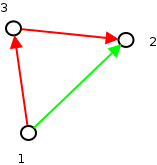
\includegraphics[width=2.5cm]{gfx/triangle_inequality}
        \caption{Dreiecksungleichung}
        \label{img:triangle_inequality}
\end{figure}

\subsection{Motivation}
Mich fasziniert, dass die Problembeschreibung sehr einfach ist, die Lösung jedoch äusserst schwierig.
Ausserdem lassen sich viele Überlegungen mit Papier und Stift aufzeichnen, ohne das ein Computer benötigt wird. 
Abbildung \ref{img:simple_tsp} zeigt ein 6 Städte TSP, eine mögliche Route ist dabei blau markiert. Offensichtlich ist es nicht die optimale Route. Das Bild zeigt jedoch, wie einfach man das Problem für kleine Instanzen analysieren kann, selbst ohne einen Rechner zu benutzen.

\begin{figure}[H]
        \centering
        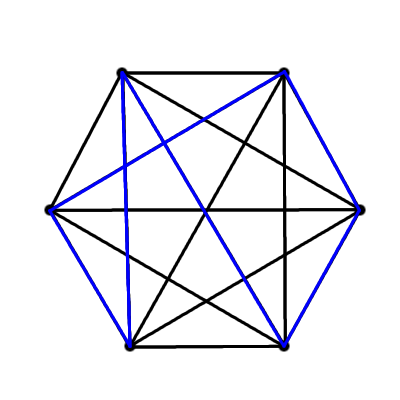
\includegraphics[width=4cm]{gfx/simple_tsp}
        \caption{6 Städte TSP}
        \label{img:simple_tsp}
\end{figure}

\newpage
\section{Traveling Salesman Problem (TSP)}
\label{s:traveling_salesman_problem}
Dieser Abschnitt gibt einen Überblick zum Traveling Salesman Problem. Als Erstes wird die Problemstellung erklärt und anschliessend der geschichtliche Hintergrund erläutert. Nach einer kurzen Beschreibung zur NP-Vollständigkeit des Problems, wird erklärt, wie das Problem modelliert werden kann. Da es neben dem in dieser Arbeit vorgestellten Algorithmus viele weitere Möglichkeiten gibt, ein TSP zu lösen, werden einige exakte und heuristische Lösungsverfahren kurz beschrieben.

\subsection{Problembeschreibung}
Die Problemstellung ist simple: Es soll eine Rundreise durch eine Anzahl Städte gefunden werden und zwar so, dass der Handlungsreisende wieder an seinen Ausgangspunkt zurückkehrt und die zurückgelegt Strecke möglichst kurz ist.

\subsection{Geschichte}
Der Urheber der Bezeichnung "`Traveling Salesman Problem"' ist nicht genau bekannt. Es ist jedoch klar, dass damit das Auffinden der kürzesten Rundreise eines Handlungsreisenden gemeint ist.\footnote{vgl. \cite{applegate06} Seite 1-3} 1983 publizierte Heiner Müller-Merbach in seinem Paper\cite{mueller83} einen Ausschnitt aus dem Buch "`Der Handlungsreisende – wie er sein soll und was er zu thun hat, um Aufträge zu erhalten und eines glücklichen Erfolgs in seinen Geschäften gewiß zu sein – von einem alten Commis-Voyageur"' in dem die Wichtigkeit einer guten Route beschrieben:  
\begin{quotation}
Die Geschäfte führen Handlungsreisende bald hier, bald dort hin, und es lassen sich nicht füglich Reiserouten angeben, die für alle vorkommende Fälle passend sind: aber es kann durch eine zweckmäßige Wahl und Eintheilung der Tour, manchmal so viel Zeit gewonnen werden, dass wir es nicht glauben umgehen zu dürfen, auch hierüber einige Vorschriften zu geben. Ein Jeder möge so viel davon benutzen, als es seinem Zwecke für dienlich hält: so viel glauben wir aber davon versichern zu dürfen, daß es nicht wohl thunlich sein wird, die Touren durch Deutschland in Absicht der Entfernungen und, worauf der Reisende hauptsächlich zu sehen hat, des Hin- und Herreisens, mit mehr Oekonomie einzurichten. Die Hauptsache besteht immer darin: so viele Orte wie möglich mitzunehmen, ohne den nämlichen Ort zweimal berühren zu müssen.
\end{quotation}

Auch wenn das Problem in diesem Buch nicht mathematisch analysiert wird, beschreibt der Text das Traveling Salesman Problem. 

Eine der ersten mathematischen Analysen des Problem stammen aus dem Jahr 1757 vom berühmten Schweizer Mathematiker Leonard Euler. Er veröffentlichte ein Paper, in dem er eine Lösung zur "`Knights Tour"' vorstellte. Bei der "`Knights Tour"' soll auf einem Schachbrett mit dem Springer eine Folge von Sprüngen gefunden werden, so dass jedes Feld genau einmal besucht wird und der Springer am Ende wieder auf seinem Startfeld steht.

Dieses Problem kann als TSP formuliert werden. Die Wegkosten zu den mittels einem Springer erreichbaren Felder sind 0, die Kosten zu den nicht erreichbaren Felder sind 1.\footnote{vgl. \cite{applegate06} Seite 8-10}

\medskip

Einer der bedeutensten frühen Forscher auf dem Gebiet, Merril Flood, sagte in einem Interview, dass der Begriff "`Traveling Salesman Problem"' in den 1930er Jahren als Synonym für das "`48 States Problem"' von Hassler Whitney an der Princeton Universität verwendet wurde. Wer genau die Bezeichnung eingeführt habe, wisse er jedoch nicht.\cite{interview_merrill_flood84}

Abschliessend ist somit nicht auszumachen, wann genau die Forschung auf dem Gebiet des Traveling Salesman Problems begonnen hat.

\medskip

Ein erster Meilenstein im Bezug auf die Lösung des Traveling Salesman Problems gelang George Dantzig, Ray Fulkerson und Selmer Johnson 1954, als sie ein 49 Städte TSP lösen konnten. Die gelöste Instanz beinhaltet Städte aus allen damaligen Bundesstaaten der USA, plus Washington D.C. Das Problem konnte gelöst werden, in dem die Städte Baltimore, Wilmington, Philadelphia, Newark, New York, Hartford und Providence entfernt wurden. Da die Route des neuen TSP durch die entfernten Städte führte, war die optimale Lösung gefunden.

In den 1960er und 1970er beschäftigten sich immer mehr Wissenschaftler mit dem Problem. Richard M. Karp konnte 1972 die NP-Vollständigkeit des Hamiltonkreisproblems beweisen, was die NP-Vollständigkeit des Traveling Salesman Problems impliziert.
%TODO: Quelle

1977 wurde ein 120 Städte TSP von Martin Grötschel gelöst. Die Route beinhaltete Städte im damaligen Westdeutschland.

Im Jahre 1987 wurden gleich drei bedeutende Instanzen gelöst: Ein 532 Städte TSP von Padberg und Rinaldi, ein 666 Städte TSP von Grötschel und Holland und das 2392 Städte TSP, wiederum von Padberg and Rinaldi.\footnote{vgl. \cite{applegate06} S. 50-51}

Anfang der 1990er Jahre begannen David Applegate, Robert E. Bixby, Vašek Chvátal und William J. Cook mit der Entwicklung von Concorde. Seit 1992 wurden immer grössere Instanzen mit Hilfe von Concorde gelöst. Die grössten Erfolg von 1992-2006 sind in Tabelle \ref{tab:concorde_history} ersichtlich.\footnote{\cite{applegate06} Seite 53}

        \begin{table}[H]
                \centering
                \begin{tabular}{| l | r | l |}
                    \hline
                        Jahr    & Anzahl Städte & Bemerkung                 \\ \hline
                        1992    & 3'038         &                           \\ \hline
                        1993    & 4'461         &                           \\ \hline
                        1994    & 7'397         &                           \\ \hline
                        1998    & 13'509        &                           \\ \hline
                        2001    & 15'112        &                           \\ \hline
                        2004    & 24'978        &                           \\ \hline
                        2004    & 33'810        & Concorde mit Domino Party \\ \hline
                        2006    & 85'900        & Concorde mit Domino Party \\ \hline
                \end{tabular}
                \caption{mit Concorde gelöste TSP Instanzen}
                \label{tab:concorde_history}
        \end{table}

Das 2006 gelöst 85'900 Städte Problem ist das grösste bisher gelöste TSP. Zur Berechnung wurde ein Cluster von 64 2.4-GHz AMD Opteron Prozessoren und 192 Xeon Prozessoren benötigt.

Die nächste Herausforderung ist das so genannte "`World TSP"', es beinhaltet 1'904'711 Städte. Die beste bekannte Lösung stammt von Keld Helsgaun. Mit Concorde konnte berechnet werden, dass die Lösung von Helsgaun maximal 0.058\% länger ist, als die optimale Lösung.

\newpage

\subsection{NP-Vollständigkeit}
Das Traveling Salesman Problem ist eines der bekanntesten NP\footnote{Nondeterministic Polynomial-Time}-Vollständigen Probleme. 

Es wird auch in der Liste von Karps 21 NP-Vollständigen Problemen aufgeführt. Die 1972 veröffentlichte List\cite{karp72} enthält sowohl das gerichtete, wie auch das ungerichtete Hamiltonkreisproblem (das TSP ist ein Spezialfall des Hamiltonkreisproblem). 

\medskip

In Hopcrofts "`Einführung in die Automatentheorie, formale Sprachen und Komplexitätstheorie"' findet sich folgende Definition:\footnote{\cite{hopcroft02} Seite 432}

Sei $L$ eine Sprache (eine Problem) in $\mathcal{NP}$. Wir sagen $L$ ist NP-vollständig, wenn folgende Aussagen über $L$ wahr sind:
\begin{itemize}
    \item L ist in $\mathcal{NP}$ enthalten.
    \item Für jede Sprache $L'$ in $\mathcal{NP}$ existiert eine polynomiale Reduktion von $L'$ auf $L$.
\end{itemize}

%TODO: Genauere Beschreibung, warum TSP NP-Vollständig
%Oder anders ausgedrückt: Wenn wir von einem Problem $L$ wissen, dass es in $\mathcal{NP}$ ist und wir unser Problem $P$ mit polynomialen Zeitaufwand auf das Problem $L$ abbilden können, dann ist $P$ NP-vollständig.

\subsection{Modellierung}
Das Problem des Handlungsreisenden wird für diese Arbeit (wie in vielen anderen Beispielen) als Graph modelliert. Dabei repräsentieren die Knoten die Städte und die Kanten die Kosten um von einer Stadt zur nächsten zu gelangen. Dabei sind die Kosten um von $A$ nach $B$ zu gelangen äquivalten zu den Kosten von $B$ nach $A$, es handelt sich also um einen ungerichteten Graphen.

Da alle Möglichen Routen berücksichtigt werden müssen, wird ein Vollständiger Graph verwendet, d.h. jeder Knoten ist mit jedem Knoten verbunden.

\subsection{Lösungsverfahren}
Neben dem hier vorgestellten Algorithmus existieren viele weitere Lösungsverfahren. Zum Vergleich sollen einige dieser Verfahren kurz vorgestellt werden.

\subsubsection{Exakte Lösungsverfahren}
\begin{flushleft}
\textbf{Brute Force}

Bei dieser Methode werden alle möglichen Kombinationen berechnet, bei jeder Berechnung wird verglichen, ob die Lösung besser ist, als die bisher berechneten Lösungen. Offensichtlich ist dieses Vorgehen äusserst ineffizient. Für 20 Städte müssen 2'432'902'008'176'640'000 (20!) Permutationen berechnete werden, dies entspricht $\approx$ $10^{18}$, also $\approx2.5$ Trillionen Möglichkeiten. Das Lösungsverfahren hat somit eine Laufzeit von $\mathcal O(n!)$.
%TODO: Genauere Ausführung: symmetrisch, asymmetrisch

\end{flushleft}

\medskip

\begin{flushleft}
\textbf{Branch-and-Cut}

Die Branch-and-Cut Verfahren ist eine Kombination des Schnittebenenverfahrens mit dem Branch-and-Bound Verfahren. 
Beim Schnittebenenverfahren wird das Problem als lineares Programm formuliert und anschliessend die Lösung der LP-Relaxierung durch hinzufügen weiterer Ungleichungen verbessert.
Beim Brach-and-Bound Verfahren wird die Lösungsmenge in Teilmengen aufgeteilt, so dass nicht optimale Bereiche der Lösungsmenge nicht berücksichtigt werden. Dies hat den Vorteil, dass nicht alle möglichen Lösungen durchprobiert werden müssen.
Die beiden Verfahren werden bei Brach-and-Cut kombiniert. Dabei wird erst das Schnittebenenverfahren angewandt und anschliessend das Branch-and-Bound Verfahren.\footnote{vgl. \cite{applegate06} Seite 117-124}

Das Branch-and-Cut Verfahren wird nicht nur beim Problem des Handlungsreisenden angewandt, sondern findet allgemein Anwendung in LP-Solvern\footnote{Löser für lineare Programme}.
%TODO: Beschreibung OK?

\end{flushleft}

\subsubsection{Heuristische Lösungsverfahren}
\begin{flushleft}
\textbf{Nearest-Neighbor-Heuristik}

Die Nearest-Neighbor-Heuristik startet an einem beliebigen Knoten, im nächsten Schritt wird der Nachbarknoten mit den Geringsten Kosten (also der Kante mit dem kleinsten Gewicht) besucht. Von diesem Knoten aus wird wieder der Nachbar gesucht, der mittels der Kante  mit dem geringsten Gewicht verbunden ist. Der Startknoten wird mit der letzten verbleibenden Kante erreicht.\cite{gutin02}
\end{flushleft}

\medskip

\begin{flushleft}
\textbf{Ant Colony Optimization (ACO)}

Die erste Anwendung des Ameisenalgorithmus (Ant Colony Optimization) war das Traveling Salesman Problem.\footnote{\cite{dorigo99} Seite 146}

ACO bedient sich der Beobachtung aus der Natur, dass Ameisen bei der Suche nach Futter eine Pheromonspur hinterlassen, mit deren Hilfe nachfolgende Ameisen den Weg zum Futter finden.

Wenn beispielsweise zwei Wege zu einer Futterquelle führen, so werden zu Beginn beide Wege mit der selben Wahrscheinlichkeit gewählt. Auf dem kürzeren der beiden Wege ist die Pheromonspur nach einer Zeitspanne $t$ allerdings höher, da eine Ameise die diesen Weg wählt nach einem Zeitraum $t$ bereits zurückkehrt, während eine Meise auf dem längeren Weg noch nicht zurück ist.

Die Pheromonkonzentration erhöht nun die Wahrscheinlichkeit, dass ein Weg gewählt wird. Somit werden die kürzeren Wege bevorzugt. \cite{dorigo99}

\end{flushleft}

\medskip

\begin{flushleft}
\textbf{MST-Heuristik}

Die MST-Heuristik garantiert eine Tour, die maximal doppelt so lang ist, wie die optimale Tour. Der Algorithmus funktioniert wie folgt:\footnote{vgl. \cite{teschl06} Seite 460}

\begin{enumerate}
    \item Minimalen Spannbaum erstellen
    \item Alle Kanten verdoppeln
    \item Eulerkreis ablaufen und dabei bereits besuchte Knoten überspringen
\end{enumerate}

\end{flushleft}
\newpage
\section{Win/Win Strategie}
Das Konzept der Win/Win Strategie für Näherungsalgorithmen wurde von H.J. Böckenhauer, Ralf Klasing, Tobias Mömke und Monika Steinová im Paper "`Improved approximations for TSP with simple precedence constraints"'\cite{boeckenhauer10} vorgestellt.  Auch D. Eppstein veröffentlichte in "`Paired approximation problems and incompatible inapproximabilities"`\cite{eppstein10} dieses Konzept. Er benutzt allerdings die Bezeichnung "`paired approximation"'.


\subsection{Grundidee}
Die Win/Win Strategie basiert darauf, dass für zwei verwandte Probleme Algorithmen $A_1$ und $A_2$ existieren und das eine Instanzen, für die $A_1$ eine schlechte Lösung liefert, $A_2$ eine gute Lösung liefert. Dass also die Worst-Case Instanzen der beiden Algorithmen disjunkt sind.

\subsection{Anwendung für das Traveling Salesman Problem}
Das Traveling Salesman Problem, welches im Abschnitt \ref{s:traveling_salesman_problem} bereits beschrieben wurde ist eng Verwandt mit dem Hamiltonpfadproblem. Beim Hamiltonpfadproblem wird nicht eine Rundreise gesucht, bei der Start und Ziel in der selben Stadt sind, sondern eine Reise durch $n$ Städte, bei der Start $s$ und Ziel $t$ in zwei verschiedenen Städten liegen. Wenn man beim HPP für $s$ und $t$ die selbe Stadt wählt, entspricht dies einem TSP.

Der Christofides Algorithmus ist die Heuristik mit der besten Gütegarantie für das Traveling Salesman Problem. Die Rundreise, die mittels Christofides Algorithmus berechnet wird, ist maximal 1/2\% länger, als die optimale Route. Diese obere Grenze konnte seit der Veröffentlichung vor über 30 Jahren nicht verbessert werden.

Für das Hamiltonpfadproblem ist der Hoogeveen Algorithmus die beste bekannte Heuristik, der gefundene Pfad ist maximal 2/3 länger als der optimale Pfad. Seit über 20 Jahren konnte kein Algorithmus gefunden werden, der eine tiefere obere Grenze garantiert.\cite{moemke11}

Für die Win/Win Strategie bedeutet dies nun, dass Instanzen, für die der Christofides Algorithmus schlechte Näherungen liefert, der Hoogeveen Algorithmus gute Lösungen liefert, die signifikant unterhalb der oberen Schranke liegen.

\newpage
\section{Algorithmen}
\label{s:algorithmen}
\subsection{Notation}
Für die folgenden Algrithmen sei $G$ ein Graph, $V$ dessen Knoten, $E$ die Kanten und $E(G)$ die Anzahl Kanten des Graphen.

\subsection{Win/Win Algorithmus}
Der verwendete Algorithmus berechnet sowohl den Hamiltonpfad, wie auch den Hamiltonkreis für einen gegebenen Graphen $G$. 
Die Berechnung basiert auf dem Paper "`Structural Properties of Hard Metric TSP Inputs"'\cite{moemke11} (der Algorithmus wurde bereits im Paper "`Improved Approximations for TSP with Simple Precedence Constraints"'\cite{boeckenhauer10} vorgestellt):

\begin{algorithm}
    \caption{Hamiltonpfad und -kreis \cite{moemke11}}
    \label{alg:hp_hc}
\textbf{Eingabe:} Ein vollständiger Graph $G = (V,E)$, eine metrische Kostenfunktion $c: E \rightarrow \mathbb{Q}^+$ und zwei Knoten $s$ und $t$.
    \begin{enumerate} \item Minimalen Spannbaum $T$ von $G$ berechnen.
        \item Minimales Perfect Matching $M_C$ der ungeraden Knoten des minimalen Spannbaumes $T$ von $G$ berechnen.
        \item Minimales Perfect Matching $M_P$ der ungeraden Knoten des Multigraphen $T$ + \{$s$, $t$\} von $G$ berechnen.
        \item Die Eulertour Eul$_C$ des Multigraphen T $\cup$ $M_C$ und den Eulerpfad Eul$_P$ des Multigraphen T $\cup$ $M_P$ berechnen.
        \item Eul$_C$ zu einer Hamiltontour $H_C$ und Eul$_P$ zu einem Hamiltonpfad $H_P$ kürzen.
    \end{enumerate}
\textbf{Ausgabe:} $H_C$ and $H_P$.

\end{algorithm}

Nachfolgend werden die einzelnen Schritte des Algorithmus \ref{alg:hp_hc} genauer beschrieben. Dabei wird erläutert, welcher Algortihmus für den jeweiligen Schritt verwendet wird und wie dieser funktioniert.

\subsection{Eingabe}
Für die Berechnung wird ein vollständiger Graph erstellt, d.h. jeder Knoten des Graphen ist mit jedem anderen Knoten verbunden.

Damit der Hamiltonpfad berechnet werden kann, wird ein Startpunkt $s$ und ein Endpunkt $t$ benötigt.

\subsection{Minimaler Spannbaum - Algorithmus von Prim}
Auf dem als Eingabe erstellten vollständigen Graphen wird nun ein minimaler Spannbaum (MST) berechnet. Zur Berechnung des MST wird der Algorithmus von Prim genutzt.

Um den minimalen Spannbaum zu finden werden folgende Schritte abgearbeitet\footnote{vgl. \cite{cormen07} Seiten 574-577}:

%TODO: Wie soll der Algorithmus beschrieben werden?
\begin{algorithm}[H]
    \renewcommand{\algorithmicrequire}{\textbf{Eingabe:}}
    \renewcommand{\algorithmicensure}{\textbf{Ausgabe:}}
    \caption{minimaler Spannbaum}

    \begin{algorithmic}[1]
    \REQUIRE Ein vollständiger Graph $G$
        \STATE Wähle einen zufälligen Startknoten $v_0$ aus $G$
        \STATE Suche die Kante $e_0$ mit dem minimalen Gewicht, die mit $v_0$ verbunden ist (falls mehrere mit $v_0$ verbindene Kanten das minimale Gewicht aufweisen, wähle zufällig eine aus)
        \STATE Füge $e_0$ zum minimalen Spannbaum $M$ hinzu
        \STATE Entferne die Kante $e_0$ aus $G$

        \WHILE{$E(G) \ge 0$}
            \STATE Suche die Kante $e_n$ mit dem minimalen Gewicht, die mit $M$ verbunden ist (falls mehrere mit $M$ verbindene Kanten das minimale Gewicht aufweisen, wähle zufällig eine aus)
            \STATE Füge $e_n$ zum minimalen Spannbaum $M$ hinzu
            \STATE Entferne die Kante $e_n$ aus $G$
        \ENDWHILE
    \ENSURE minimaler Spannbaum $M$
    \end{algorithmic}
\end{algorithm}

\begin{figure}[H]
        \centering
        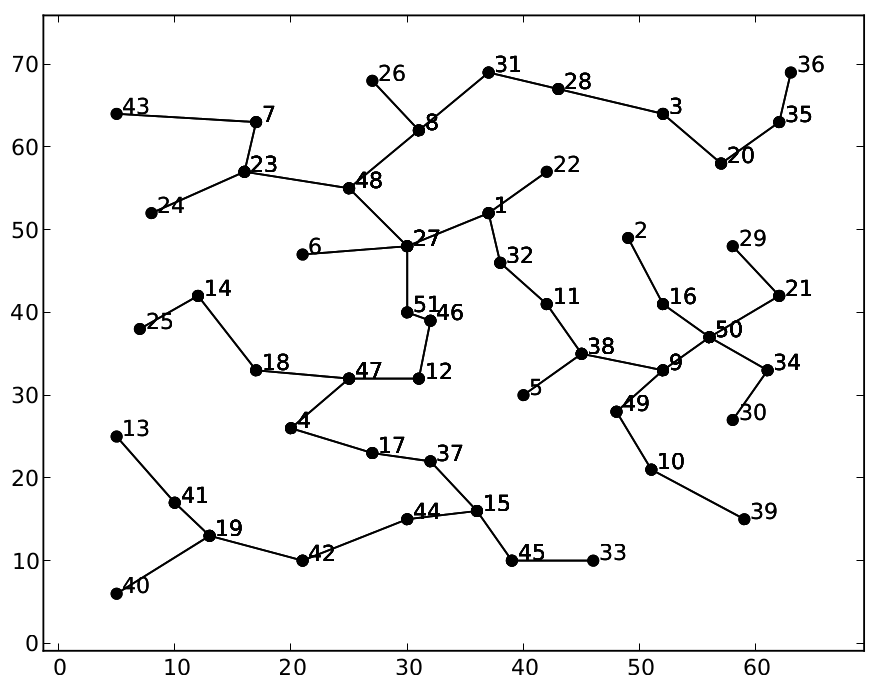
\includegraphics[width=14cm]{gfx/eil51_mst}
        \caption{Minimaler Spannbaum der TSP Instanz eil51 (TSPLIB)}
        \label{img:eil51_mst}
\end{figure}


%TODO: Bilder einfügen, um die Vorgehensweise aufzuzeigen?

\subsection{Minimales Perfektes Matching - Blossom V}
%TODO: Genauer beschreiben
Das minimale Perfekt Matching wird mittels Blossom V Algorithmus berechnet. Der Blossom V Algortihmus ist eine Weiterentwicklung des bekannten Blossom Algorithmus, der 1965 von Edmonds vorgestellt wurde.
Für diesen Algorithmus wird eine bestehende Implementation verwendet. 

\begin{figure}[H]
        \centering
        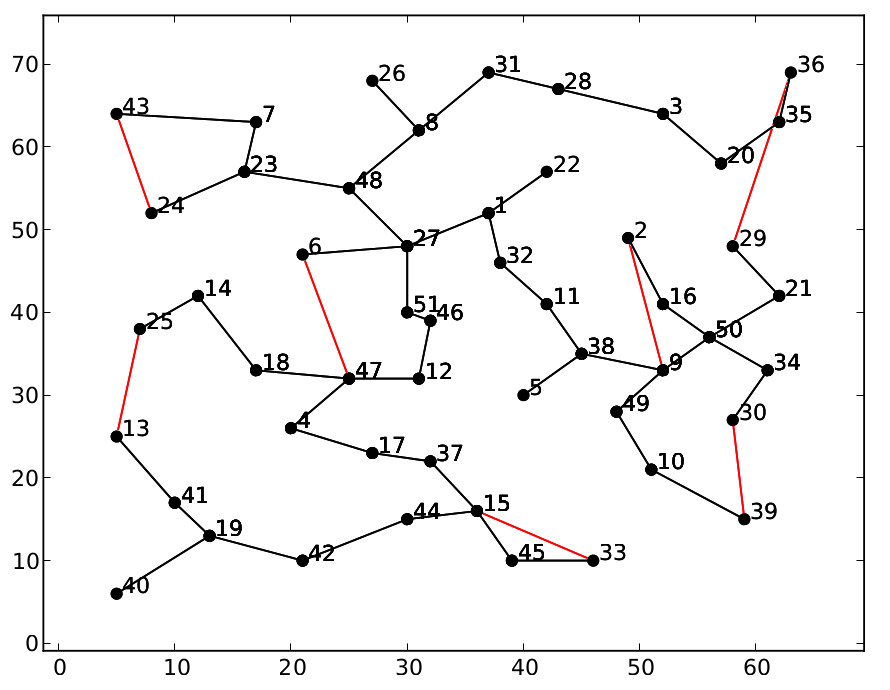
\includegraphics[width=14cm]{gfx/eil51_pm}
        \caption{Minimales Perfect Matching (rot) auf den ungeraden Knoten des MST (schwarz)}
        \label{img:eil51_pm}
\end{figure}

\subsection{Eulerkreis - Hierholzer}
Die Berechnung des Eulerkreises wird mittels Algorithmus von Hierholzer zurück. Dieser wurde 1873 in der postum veröffentlichten Arbeit "`Über die Möglichkeit, einen Linienzug ohne Wiederholung und ohne Unterbrechung zu umfahren"'\cite{hierholzer73} beschrieben.

Der Algorithmus basiert auf der Idee, dass, wenn man in einem eulerschen Graphen einen beliebigen Kreis findet, die verbleibenden Kanten wiederum einen Kreis enthalten. Somit werden die gefundenen Kreise zusammengefügt, bis schlussendlich alle Kanten im Kreis enhalten ist und somit der Eulerkreis gefunden wurde.\footnote{vgl. \cite{krumke05} Seiten 46-48}

%TODO: Ist die beschreibung verständnlich?
\begin{algorithm}[H]
    \renewcommand{\algorithmicrequire}{\textbf{Eingabe:}}
    \renewcommand{\algorithmicensure}{\textbf{Ausgabe:}}
    \caption{Algorithmus von Hierholzer}

    \begin{algorithmic}[1]
    \REQUIRE Graph $G$, dessen Knoten alle einen geraden Grad aufweisen
        \STATE Wähle einen beliebigen Startknoten $v_0$
        \STATE Erstelle einen Kreis $K$ ausgehend von $v_0$
        \STATE Entferne alle Kanten von $K$ aus $G$
        \WHILE{$E(G) \ge 0$}
            \STATE Suche Knoten $v_n$ dessen Grad $\ge 0$
            \STATE Erstelle einen Kreis $K_n$ ausgehend von $v_n$
            \STATE Füge $K_n$ zu $K$ hinzu: Alle Knoten von $K_n$ an Stelle des Startknotens von $K_n$ in der korrekten Reihenfolge in $K$ einfügen
            \STATE Entferne alle Kanten von $K_n$ aus $G$
        \ENDWHILE
    \ENSURE Eulerkreis $K$
    \end{algorithmic}
\end{algorithm}

\begin{figure}[H]
        \centering
        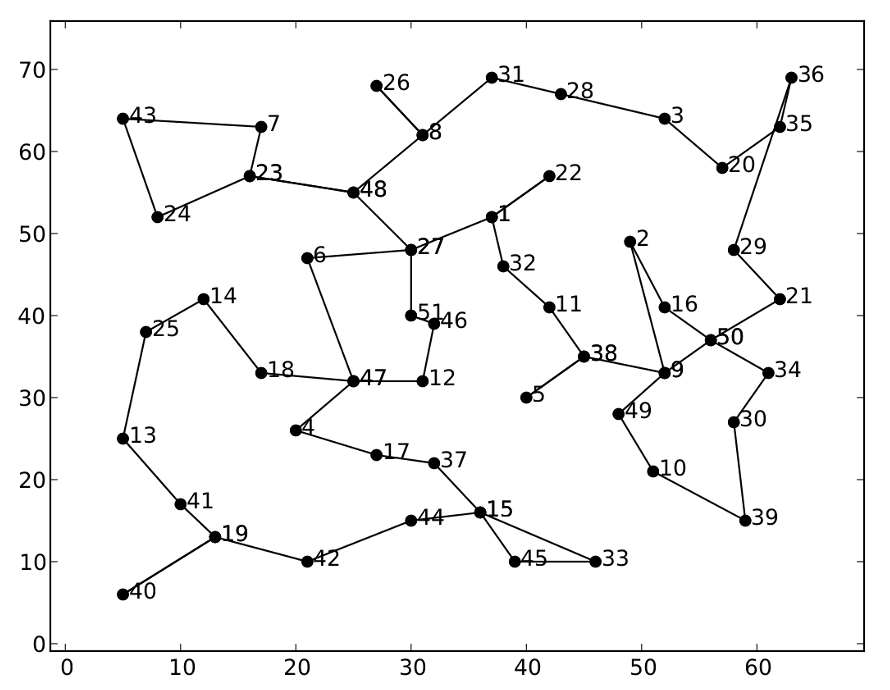
\includegraphics[width=14cm]{gfx/eil51_euler}
        \caption{Eulerkreis}
        \label{img:eil51_euler}
\end{figure}

%TODO: Weitere Bilder einfügen, um die Vorgehensweise aufzuzeigen?


\subsection{Kürzung Eulerkreis/-pfad zu Hamiltonkreis/-pfad}
Die kürzung des Eulerkreises bzw. des Eulerpfades werden in der Liste der besuchten Knoten alle doppelten Einträge gelöscht.

\begin{algorithm}[H]
    \renewcommand{\algorithmicrequire}{\textbf{Eingabe:}}
    \renewcommand{\algorithmicensure}{\textbf{Ausgabe:}}
    \caption{Kürzung Eulerkreis/-pfad zu Hamiltonkreis/-pfad}

    \begin{algorithmic}[1]
    \REQUIRE Liste $L$ mit den Knoten des Eulerkreises/-pfades 
    \FOR{$i = 1 \to len(L)$}
        \IF{$L[i]$ not in $H$}
            \STATE Füge $L[i]$ zu $H$ hinzu
        \ENDIF
    \ENDFOR
    \ENSURE Hamiltonkreis/-pfad $H$
    \end{algorithmic}
\end{algorithm}

\begin{figure}[H]
        \centering
        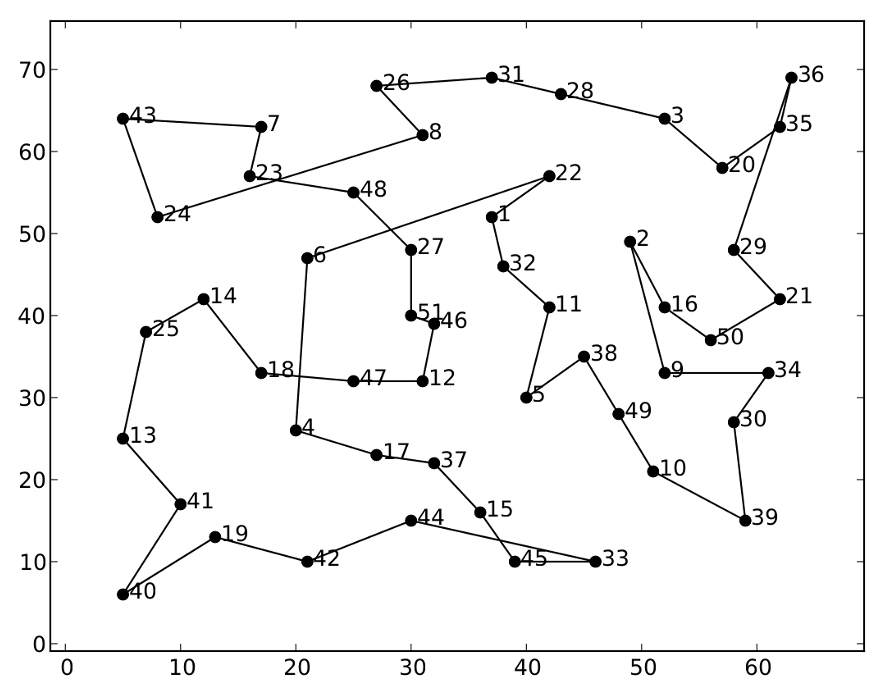
\includegraphics[width=14cm]{gfx/eil51_tour}
        \caption{Hamiltonkreis nach Kürzung des Eulerkreises}
        \label{img:eil51_tour}
\end{figure}

\newpage
\section{Implementation}
Der gesamte Algorithmus ist in Python 3 implementiert. Lediglich der Blossom V Algorithmus, für welchen eine bestehende Implementation verwendet wird, ist in C++ implementiert.

Für die Knoten, Kanten und Graphen werden eigene Objekte erstellt, die nachfolgend genauer beschrieben werden. 

%TODO: Einleitung: Verwendete Programmiersprache, Unittesting, etc.
\subsection{Datenstrukturen}
\subsubsection{Knoten}
Jeder Knoten hat eine eindeutige ID die vom System vergeben wird. Zudem erhält jeder Knoten eine Nummer und eine Liste von Koordinaten, diese Informationen werden aus dem TSP-File gelesen. Zusätzlich ist es möglich, ein Label anzugeben, um weitere Informationen zu speichern.

Die Koordinaten sind als Liste implementiert, um unabhängig von der Dimension der Instanz die benötigten Informationen speichern zu können.

Damit die Knoten in einem \emph{dictionary}\footnote{zu vergleichen mit einer Hashtable in Java} gespeichert werden können, implementiert dieses Objekt die \emph{hash} Funktion. Dazu wird die ID des Objekts mit der von Python zur Verfügung gestellten Funktion gehashed.

\subsubsection{Kante}
Kanten werden ebenfalls durch eine eindeutige ID, die durch das System vergeben wird, identifiziert.

Eine Kante setzt sich zusammen aus zwei Knoten und einer Gewichtung der Kante. Die Gewichtung wird auf die nächste Ganzzahl gerundet. Dies entspricht der Spezifikation der TSPLIB.\footnote{\cite{reinelt95} Seite 6}

Um Kanten sortieren zu können, wird die Funktion \texttt{\textunderscore\textunderscore lt\textunderscore\textunderscore} implementiert. Diese vergleicht eine gegebene Kante $E1$ mit einer zweiten $E2$ und gibt \texttt{True} zurück, wenn $E1 < E2$.

Die Funktion \texttt{\textunderscore\textunderscore eq\textunderscore\textunderscore} prüft, ob zwei Kanten identisch sind, in dem die IDs der Kanten verglichen werden.

\subsubsection{Graph}
Die zentrale Datenstruktur für die Berechnungen ist der Graph. In Tabelle \ref{tab:impl_graph} werden die wichtigsten Funktionen beschrieben.

Wichtige für eine effiziente Funktionsweise ist die Speicherung der Knoten und Kanten. Die Knoten werden in einem mehrdimensionalen \emph{dictionary} gespeichert. Die Knoten fungieren im ersten \emph{dictionary} als Keys. Dieser Key zeigt auf ein weiteres \emph{dictionary}, der Key dieses \emph{dictionary} ist wiederum ein Knoten der auf eine Liste von Kante zeigt, die die beiden Knoten verbinden.

Diese Implementation hat den Vorteil, dass direkt auf Knoten, Kanten und Nachbarknoten zugegriffen werden kann. Da zwei Knoten durch mehrere Kanten verbunden sein können, werden die Kanten in einer Liste gespeichert.

\begin{table}[H]
                \centering
                \begin{tabular}{| p{3cm} | p{3cm} | p{3cm} | p{5cm} |}
                    \hline
                    \textbf{Name}                                               & \textbf{Parameter}        & \textbf{Rückgabewert}     & \textbf{Beschreibung} \\ \hline
                    \texttt{add\textunderscore node}                            & Knoten $v_n$              &                           & Fügt den Knoten $v_n$ zum Graphen hinzu \\ \hline
                    \texttt{add\textunderscore edge}                            & Kante  $e_n$              &                           & Fügt die Kante $e_n$ zum Graphen hinzu \\ \hline
                    \texttt{remove\textunderscore edge}                         & Kante  $e_n$              &                           & Entfernt die Kante $e_n$ aus dem Graphen \\ \hline
                    \texttt{neighbour\textunderscore nodes}                     & Knoten $v_n$              & Liste von Knoten          & Gibt alle mit dem Knoten $v_0$ \newline verbundenen Knoten zurück\\ \hline
                    \texttt{neighbour\textunderscore edges}                     & Knoten $v_n$              & Liste von Kanten          & Gibt alle mit dem Knoten $v_0$ \newline verbundenen Kanten zurück\\ \hline
                    \texttt{contains\textunderscore node}                       & Knoten $v_n$              & \texttt{True/False}       & Gibt \texttt{True} zurück, wenn der Graph den Knoten enthält, sonst \texttt{False} \\ \hline
                    \texttt{contains\textunderscore edge}                       & Knoten $v_n$ und $v_m$    & \texttt{True/False}       & Gibt \texttt{True} zurück, wenn der Graph die Kante enthält die $v_n$ und $v_m$ verbindet, sonst \texttt{False} \\ \hline
                    \texttt{edge\textunderscore by\textunderscore nodes}        & Knoten $v_n$ und $v_m$    & Liste von Kanten          & Gibt die Kanten zurück, die die Knoten $v_n$ und $v_m$ verbindet \\ \hline
                    \texttt{lookup\textunderscore distance}                     & Knoten $v_n$ und $v_m$    & Liste von Gewichtungen    & Gibt die Gewichtungen der Kanten zurück die  $v_n$ und $v_m$ verbindet \\ \hline
                \end{tabular}
                \caption{Wichtige Funktionen des Objektes Graph}
                \label{tab:impl_graph}
        \end{table}



\subsection{Algorithmen}
Da die Algorithmen in Abschnitt \ref{s:algorithmen} bereits beschrieben wurden, wird hier lediglich auf die wichtigsten Punkte der Implementierung eingegangen.

\subsubsection{Minimaler Spannbaum}
Zur Erstellung des minimale Spannbaums wird nach der Wahl eines Starknotens aus den erreichbaren Kanten jeweils diejenige mit dem kleinsten Gewicht gesucht. Um dies effizient zu ermöglichen, wird die bestehende Datenstruktur \emph{Priority Queue} genutzt:

\begin{flushleft}
    Initiales Befüllen der Queue, sortierung nach Gewicht:
\end{flushleft}
\begin{verbatim}
for new_edge in graph.neighbour_edges(start_node):
    neighbour_edges.add_item(new_edge.weight, new_edge)
\end{verbatim}

\begin{flushleft}
    Wahl der nächsten Kante aus der Queue:
\end{flushleft}
\begin{verbatim}
next_edge = neighbour_edges.get_top_priority()
\end{verbatim}

\begin{flushleft}
    Hinzufügen der neuen Kanten nach bei der Iteration:
\end{flushleft}

\begin{verbatim}
next_edges = graph.neighbour_edges(next_edge.node_2)
for new_edge in next_edges:
    neighbour_edges.add_item(new_edge.weight, new_edge)
\end{verbatim}

Die Iteration wird durchgeführt, bis alle Knoten im MST enthalten sind.

\subsubsection{Perfecht Matching}
Für das Perfect Matching wird eine bestehende Implementation verwendet. Um diese zu Nutzen wird eine File mit den ungeraden Knoten aufbereitet. Bei der Berechnung werden die Angaben aus dem File gelesen und das Ergebnis in ein Output-File geschrieben.

Die Kanten, die sich durch das Matching ergeben haben, werden aus dem Output-File gelesen, als Objekte erstellt und zum Graphen hinzugefügt.

\begin{flushleft}
    Liste der Ungeraden Knoten erstellen:
\end{flushleft}
\begin{verbatim}
for node in nodes:
    if len(graph.neighbour_nodes(node)) % 2 == 1:
        odd_nodes[odd_node_nr] = node
        odd_node_nr += 1
\end{verbatim}

\begin{flushleft}
    Lesen des Output-Files, erstellen der Kanten und hinzufügen zum Graphen:
\end{flushleft}
\begin{verbatim}
        for line in f:
            node_1_odd_node_nr,node_2_odd_node_nr = line.split()
            node_1 = odd_nodes[int(node_1_odd_node_nr)] 
            node_2 = odd_nodes[int(node_2_odd_node_nr)]
            weight = graph.lookup_distance(node_1, node_2)[0]
            edge = Edge(node_1, node_2, weight)
            graph.add_edge(edge)
\end{verbatim}

\subsubsection{Eulerkreis/-pfad}
Zur Erstellung des Eulerkreises/-pfades wurden zwei Routinen erstellt. Die erste erstellt die Kreise und die zweite fügt diese zusammen, bis schlussendlich der Eulerkreis-/pfad gefunden ist.

\begin{flushleft}
    In einer Schleife wird ein Nachbarknoten des aktuellen Knotens gewählt. Die dazwischenliegende Kante wird zum Eulerkreis hinzugefügt. Falls zwischen den Knoten mehrere Kanten existieren, wird diejenige mit dem kleinsten Gewicht selektiert:
\end{flushleft}
\begin{verbatim}
neighbours = graph.neighbour_nodes(current_node)
next_node = min(list(neighbours.copy().keys()))

edge_list = graph.edge_by_nodes(current_node, next_node)
current_edge = min(edge_list)
\end{verbatim}

\begin{flushleft}
    Damit zwei Kreise (\texttt{euler} und \texttt{euler\_sub}) zusammengefügt werden können, muss über die Liste iteriert werden. So kann der korrekte Punkt zum Einfügen der zweiten Liste gefunden werden.
\end{flushleft}
\begin{verbatim}
for node in euler_tmp:
    if node == current_node and found == False:
        for node_sub in euler_sub:
            euler.append(node_sub)
        found = True
    else:
        euler.append(node)
\end{verbatim}

\begin{flushleft}
   Im Falle eines Eulerpfades an stelle des Kreises ist das Vorgehen das selbe. Wenn der Kreis gefunden wurde, wird die Kante zwischen $s$ und $t$ entfernt.
\end{flushleft}

\subsubsection{Kürzung Eulerkreis/-pfad zu Hamiltonkreis/-pfad}
Die Kürzung des Eulerkreises/-pfades zu einem Hamiltonkreis/-pfad funktioniert sehr einfach. Dazu wird wird eine neue Liste von Knoten erstellt, zu der ein Knoten hinzugefügt wird, wenn er noch nicht in der Liste vorhanden ist. Beim Hamiltonkreis wird zum Schluss der Startknoten nochmals hinzugefügt, um den Kreis zu schliessen. 

Diese Implementation hat den Vorteil, dass die Kürzung nachvollziehbar ist. Eine Alternative wäre die Implementation mittels eine Datenstruktur, die keine doppelten Einträge zulässt.

\begin{verbatim}
for node in nodes:
    if node not in nodes_shortened:
        nodes_shortened.append(node)

nodes_shortened.append(nodes_shortened[0])
\end{verbatim}

\subsection{Generierung von Instanzen}
Für die Generierung der eigenen Instanzen wird ein TSP-File mit den entsprechenden Koordinaten geschrieben.

Folgende Arten von Instanzen werden generiert:

\subsubsection{Zufällige Instanzen}
Zur Generierung von Zufälligen Instanzen sind zwei Schleifen notwendig, einmal um die Anzahl Knoten zu generieren und einmal um die Anzahl Dimensionen im euklidischen Raum zu generieren. Bei den zufälligen Instanzen werden beliebige Punkte innerhalb der gegebenen minimalen und maximalen Grenzen erzeugt:

\begin{verbatim}
for i in range(0,cities):
    print('{0}'.format(i+1), end=" ", file=f)
        for j in range(0, dimension):
            print('{0}'.format(random.randrange(min_coord,max_coord)), \
                end=" ", file=f)

    print('',file=f)
\end{verbatim}

\subsubsection{Band}
Bei der Generierung von Instanzen mit einer länglichen Verteilung werden zwei verschiedene minimale und maximale Begrenzungen eingesetzt. Für eine Achse wird dazu die eine Begrenzung verwendet, für alle anderen die zweite:

\begin{verbatim}
for i in range(0,cities):
    print('{0}'.format(i+1), end=" ", file=f)
        for j in range(0, dimension):
            if j == 1:
                print('{0}'.format(random.randrange( \
                    min_coord_height,max_coord_height)), end=" ", file=f)
            else:
                print('{0}'.format(random.randrange( \
                    min_coord_width,max_coord_with)), end=" ", file=f)

    print('',file=f)
\end{verbatim}

\subsubsection{Gruppen}
Um die Gruppen zu erzeugen, wird die Seitenlänge der Quadrate angegeben, innerhalb dieser Quadrate werden die Knoten platziert. Zusätzlich wird der Abstand zwischen den Quadraten definiert. Daraus werden die Koordinaten errechnet, hier das Beispiel, mit welchem zwei Gruppen generiert werden:

\begin{verbatim}
for i in range(0,cities):
    print('{0}'.format(i+1), end=" ", file=f)

    if i % 2 == 0:
        # x coordinate first crowd
        print('{0}'.format(random.randrange(1,width_c1)), end=" ", file=f)
        # y coordinate first crowd
        print('{0}'.format(random.randrange(1,width_c1)), end=" ", file=f)
    else:
        # x coordinate second crowd
        print('{0}'.format(random.randrange(offset,offset+width_c2)), \
            end=" ", file=f)
        # y coordinate second crowd
        print('{0}'.format(random.randrange(1,width_c2)), end=" ", file=f)

    print('',file=f)
\end{verbatim}

\subsection{Unittests}
Python unterstützt standardmässig Unittests. Diese werden verwendet, um die wichtigen Komponenten des Algorithmus zu testen.

Bei Änderungen am Quellcode werden die Unittests genutzt, um zu prüfen, ob Seiteneffekte auftreten und ob es zu Fehlern kommt.
\newpage

\section{Applikation}
In diesem Abschnitt wird die Anwendung des Programms zur Berechnung der Win/Win Strategie genauer Beschrieben.

Zur Berechnung werden die benötigten Angaben aus einer Datei im TSPLIB Format gelesen. Mittels Parameter können dann verschiedene Optionen verwendet werden.

\subsection{Input File Format}
Der Graph, der zur Berechnung verwendet wird, wird in Form eines Textfiles vom Programm gelesen. Hierzu wurde die Spezifikation der TSPLIB übernommen, mit den Einschränkungen, dass nur euklidische Distanzen als Gewichtungen erlaubt sind, nur der Typ TSP unterstützt wird und die Position der Knoten durch ihre Koordinaten im Raum definiert werden.

Das TSPLIB Format besteht aus Header-Informationen und den Koordinaten der Städte.

\begin{verbatim}
NAME : hoogeveen 
COMMENT : The Hoogeveen Graph 
TYPE : TSP 
DIMENSION : 8 
EDGE_WEIGHT_TYPE : EUC_2D
NODE_COORD_SECTION
1   49      0   
2   50      60  
3   50      1050
4   0       49  
5   1051    1050
6   1100    49  
7   1050    60  
8   1051    0   
EOF
\end{verbatim}

\subsubsection{NAME}
Name der Datei.

\subsubsection{COMMENT}
Freitext Kommentar (bspw. Name des Erstellers der Instanz)

\subsubsection{TYPE}
Die TSPLIB sieht verschiedene Typen von Problemstellungen vor, neben TSP bspw. das asymmetrische TSP (ATSP). Für den Win/Win Algorithmus wird nur der TYP TSP unterstützt.

\subsubsection{DIMENSION}
Anzahl der Städte. Diese Angabe wird genutzt, um zu prüfen ob die Anzahl der Städte im Header der tatsächlich angegebenen Anzahl der Städte entspricht.

\subsubsection{EDGE\_WEIGHT\_TYPE}
Gibt an, wie die Distanzen im Dokument abgebildet werden. Es werden ausschliesslich euklidische Distanzen unterstützt (bspw. EUC\_2D, wobei 2 die Dimension des Raumes ist).
Anhand der Dimension des Raumes wird geprüft, ob die Anzahl Spalten (die Koordinaten einer Stadt) korrekt ist.

\emph{Hinweis: Gemäss Spezifikation der TSPLIB wird nur EUC\_2D und EUC\_3D unterstützt, diese Einschränkung besteht für die Win/Win Strategie nicht.}

\subsubsection{NODE\_COORD\_SECTION}
Ab hier werden die Koordinaten der Städte angegeben. Die erste Spalte ist dabei die ID des Knotens und muss fortlaufend von 1 bis N nummeriert sein. Die darauffolgenden Spalten sind Koordinaten, eine Spalte pro Achse, bspw.

\begin{verbatim}
1   x_achse     y_achse     z_achse
2   x_achse     y_achse     z_achse
3   x_achse     y_achse     z_achse
\end{verbatim}

\subsection{Anwendung}
Die Anwendung kann von der Kommandozeile aufgerufen werden. Dabei können folgende Parameter verwendet werden.

\begin{table}[H]
        \centering
        \begin{tabular}{| l | l | l |}
            \hline
            \textbf{Parameter}          & \textbf{Beschreibung}                                         & \textbf{default}      \\ \hline
            \texttt{-f (--file)}        & File, von welchem die Instanz gelesen wird                    &                       \\ \hline
            \texttt{-s (--start)}       & Startknoten des Hamiltonpfades                                &                       \\ \hline
            \texttt{-t (--end)}         & Zielknoten des Hamiltonpfades                                 &                       \\ \hline
            \texttt{-ot (--opt-tsp)}    & Zielknoten des Hamiltonpfades                                 &                       \\ \hline
            \texttt{-oh (--opt-hpp)}    & Zielknoten des Hamiltonpfades                                 &                       \\ \hline
            \texttt{-p (--print)}       & Gibt an, ob die Knoten der Lösung ausgegeben werden sollen    & \texttt{False}        \\ \hline
        \end{tabular}
        \caption{Liste der möglichen Parameter}
        \label{tab:parameter}
\end{table}

Die Parameter \texttt{-f}, \texttt{-s}, \texttt{-t} müssen bei jedem Aufruf angegeben werden.

\subsubsection{Beispiele}
Berechnung der Instanz eil51 mit dem Startknoten 36 und dem Zielknoten 40:
\begin{flushleft}
\texttt{./bin/winwin -f data/in/eil51.tsp -s 36 -t 40}
\end{flushleft}

Berechnung der Instanz dantzig42 mit dem Startknoten 14 und dem Zielknoten 41, die Länge der optimalen TSP-Route ist 675 und die Länge der optimalen HPP-Route ist 619. Die Lösungen für das TSP und das HPP wird ausgegeben:
\begin{flushleft}
\texttt{./bin/winwin -f data/in/dantzig42.tsp -s 14 -t 41 -ot 675 -oh 619 -p}
\end{flushleft}

\section{Berechnungen}
Für die Berechnung werden einerseits Instanzen aus der TSPLIB verwendet, andererseits selbst erstellte Instanzen.
Zuerst wird das Vorgehen für die Berechnung beschrieben, anschliessend werden die verwendeten Ressourcen vorgestellt. Zum Schluss werden Berechnungen auf verschiedenen Instanzen ausgewertet.

\subsection{Vorgehen}
Um die Lösung der Win/Win Strategie mit der exakten Lösung zu vergleichen wird wie folgt vorgegangen:

\begin{itemize}
    \item Berechnung der exakten Lösung mit Concorde für das TSP 
    \item Einfügen einer Dummy-Stadt (Distanz 0 zu allen Städten)
    \item Berechnung der exakten Lösung mit Concorde für HPP 
    \item Beginn und Ende der Route werden als $s$ und $t$ verwendet
    \item Berechnung der Lösung mittels Win/Win Strategie
    \item Vergleich der Win/Win Lösung mit der exakten Lösung
\end{itemize}

Die Implementierung des Graphes als "`dictionary"' hat zur Folge, dass die Knoten nicht sortiert sind. Dies bringt einerseits massive Geschwindigkeitsvorteile, andererseits führt es aber dazu, dass bei der Berechnung der selben Instanz leicht unterschiedliche Ergebnisse berechnet werden.

Um eine möglichst repräsentative Lösung für den Vergleich zu erhalten, wird bei Instanzen, die nicht auf zufälligen Werten basieren (bspw. dantzig42, eil51, christofides, hoogeveen) der arithmetische Mittelwert aus 100 Berechnungen verwendet.

Bei Instanzen die aus zufälligen Werten erzeugt werden (bspw. random, band), werden 100 verschiedene Instanzen erzeugt, pro erzeugter Instanz wird dann eine Berechnung durchgeführt.

Zu jeder Instanz werden die Ergebnisse in einer Tabelle dargestellt und interpretiert. Bei den eigenen Instanzen wird zur Illustration jeweils eine der hundert Graphen in 2D dargestellt. Am Ende werden die Abweichungen in einer Übersichtstabelle zusammengefasst.
%TODO: Berechnung entsprechend durchführen

\subsection{Genutzte Ressourcen}
\subsubsection{Concorde}
Zur Berechnung der exakten Lösung wird die Software Concorde verwendet. Concorde wurde von David Applegate, Robert E. Bixby, Vašek Chvátal und William J. Cook, den Autoren des Buches "`Traveling Salesman Problem"'\cite{applegate06}, geschrieben.

Es ist sowohl möglich, die exakte Lösung zu berechnen, wie auch Heuristiken zu verwenden. Für diese Arbeit wurde lediglich die Berechnung der exakten Lösung verwendet.

Neben dem Kommandozeilen-Programm für Linux ist auch ein GUI für Windows verfügbar.\footnote{Download unter http://www.tsp.gatech.edu/concorde/downloads/downloads.htm}

\begin{figure}[H]
        \centering
        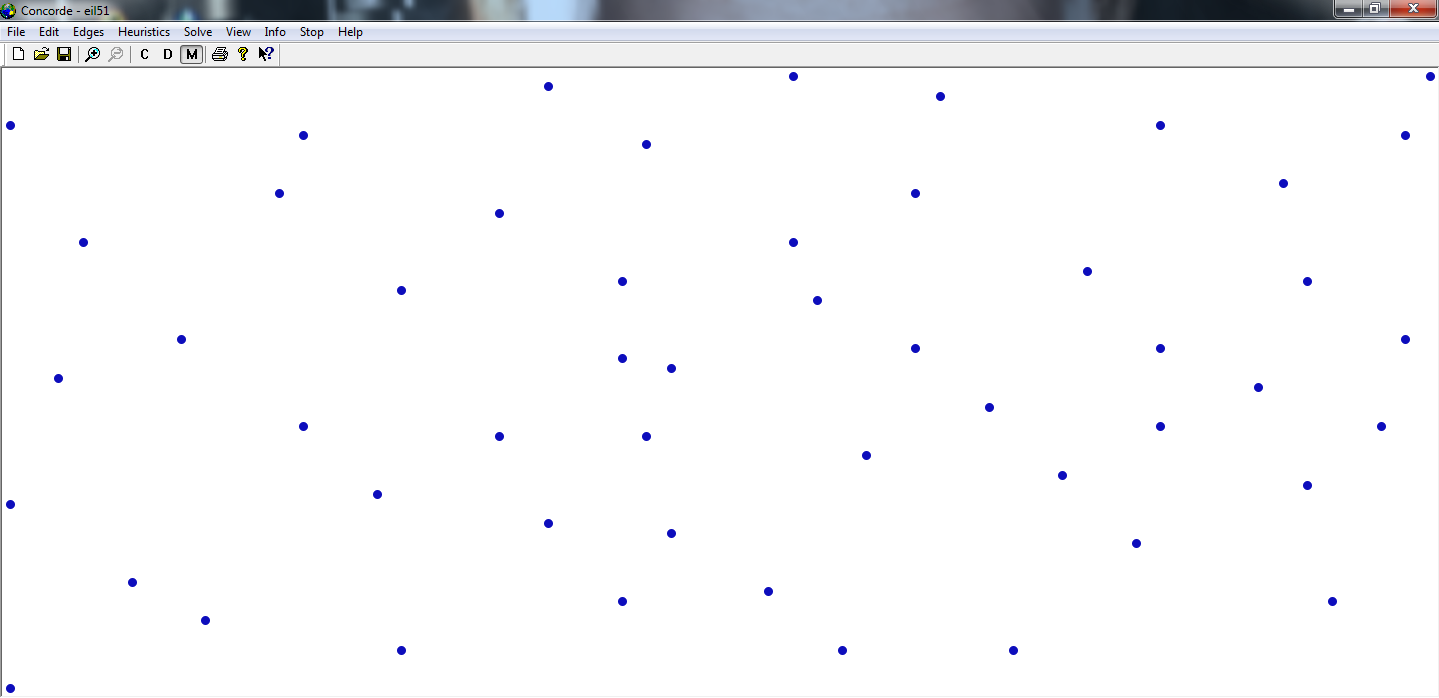
\includegraphics[width=14cm]{gfx/concorde_cities}
        \caption{Concorde stellt eil51 aus der TSPLIB garfisch dar}
        \label{img:concorde_cities}
\end{figure}

\begin{figure}[H]
        \centering
        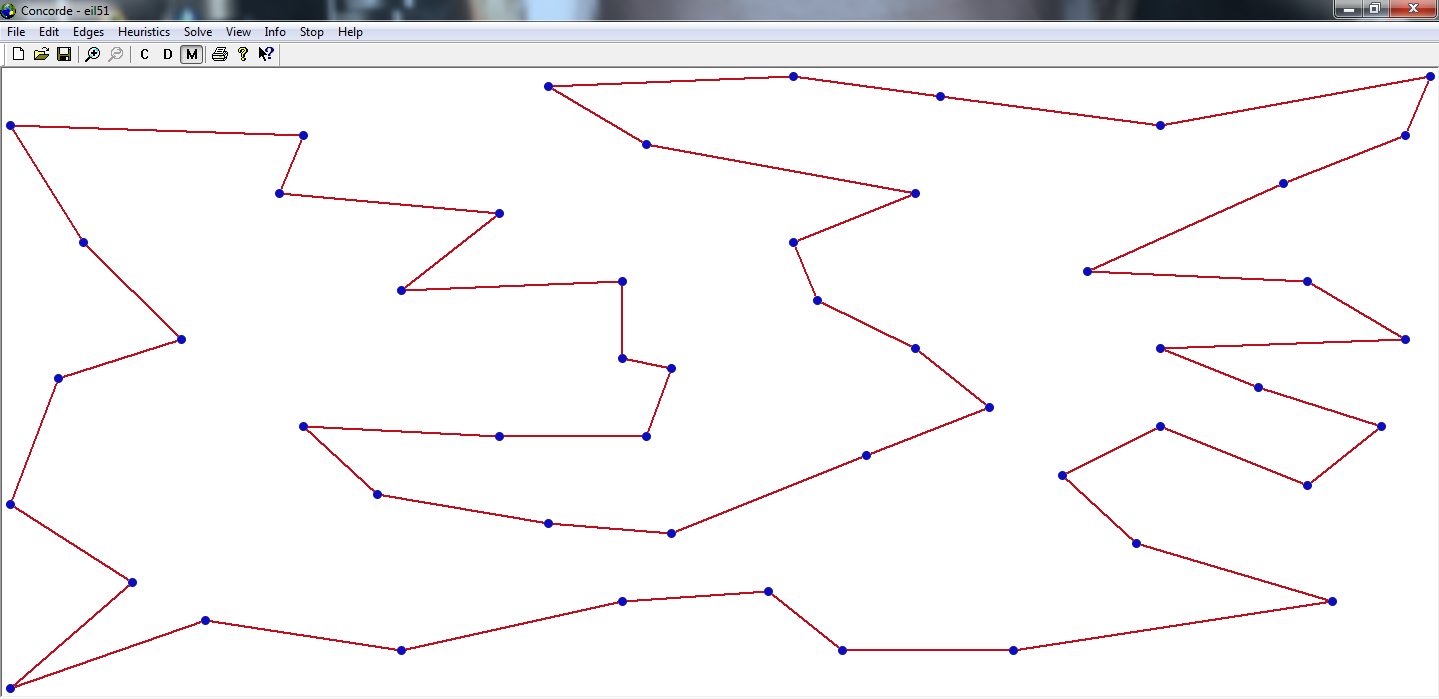
\includegraphics[width=14cm]{gfx/concorde_solution}
        \caption{Concorde hat die Lösung zu eil51 berechnet}
        \label{img:concorde_solution}
\end{figure}

\subsubsection{TSPLIB}
Die TSPLIB ist eine Sammlung von TSP-Instanzen, die 1990 von Gerhard Reinelt erstellt wurde. Sie enthält Instanzen von 14 - 85'900 Städte TSPs und ist wohl die am häufigsten genutzte Sammlung für Berechnungen des Traveling Salesman Problems.\footnote{vgl. \cite{applegate06} Seite 500-505}

Die Instanzen sind in Files abgelegt. Es werden verschiedene Formate unterstützt, unter anderem die Speicherung der Koordinaten im 2 und 3 dimensionalen euklidischen Raum und als Matrix, bei der die Elemente die Abstände zwischen den Knoten darstellt.

\subsubsection{Eigene Instanzen}
Eigene Instanzen werden verwendet, wenn bestimmte Szenarien berechnet werden sollen, die in der TSPLIB nicht verfügbar sind.

Dazu werden bestimmte Probleme von Hand erstellt. So zum Beispiel die Instanz zur Darstellung des Worst-Case des Hamiltonpfadproblems.

Neben den von Hand erstellen Problemen, wurden mittels eines einfachen Scripts Zufällige Instanzen erstellt. Diese sind entweder komplett zufällig, in dem Städte innerhalb definierten Schranken verteilt werden oder zufällig, aber mit vorgegebenen Mustern. Beispielsweise wurden Instanzen erstellt, bei denen die Städte auf der X-Ache in einem Bereich von 1-1500 liegen, auf der Y-Achse aber nur von 1-100. So werden die Städte auf einem schmalen Band verteilt.

\subsection{Auswertung TSPLIB Instanzen}

\subsubsection{dantzig42}
Die TSP-Instanz dantzig42 wurde 1954 durch G. Dantzig, R. Fulkerson und S. Johnson gelöst. Eigentlich handelt sich sich um eine Instanz mit 49 Städten, da die Berechnung mit 49 Städten zu aufwändig war, wurden 7 Städte bei der Berechnung nicht berücksichtigt. Die optimale Route führte durch die 7 entfernten Städte und war somit auch für diese optimal.

        \begin{table}[H]
                \centering
                \begin{tabular}{| l | r |}
                    \hline
                        Anzahl Städte               & 42            \\ \hline
                        Dimensionen                 & 2             \\ \hline
                        Länge optimale Lösung TSP   & 675           \\ \hline
                        Länge Win/Win Lösung  TSP   & 744.60        \\ \hline
                        Abweichung TSP              & 10.31\%       \\ \hline
                        $s$ und $t$ für HPP         & 14,41         \\ \hline
                        Länge optimale Lösung HPP   & 619           \\ \hline
                        Länge Win/Win Lösung  HPP   & 717.24        \\ \hline
                        Abweichung HPP              & 15.87\%       \\ \hline
                \end{tabular}
                \caption{Instanz dantzig42}
                \label{tab:dantzig42}
        \end{table}

Für diese Instanz liefert der Christofides Algorithmus etwas bessere Ergebnisse als der Hoogeveen Algorithmus. Die Knoten sind auf der X-Achse zwischen 3 und 174 und auf der Y-Achse zwischen 13 und 106 verteilt. Da der Minimale Spannbaum bessere Voraussetzungen für die Rundreise als für den Pfad liefert, ist die Genauigkeit für das TSP besser.

\subsubsection{bier127}
Eine Tour durch 127 Biergärten in Augsburg.

        \begin{table}[H]
                \centering
                \begin{tabular}{| l | r |}
                    \hline
                        Anzahl Städte               & 127           \\ \hline
                        Dimensionen                 & 2             \\ \hline
                        Länge optimale Lösung TSP   & 118282        \\ \hline
                        Länge Win/Win Lösung  TSP   & 133740.98     \\ \hline
                        Abweichung TSP              & 13.06\%       \\ \hline
                        $s$ und $t$ für HPP         & 98, 107       \\ \hline
                        Länge optimale Lösung HPP   & 109028        \\ \hline
                        Länge Win/Win Lösung  HPP   & 123598.08     \\ \hline
                        Abweichung HPP              & 13.36\%       \\ \hline
                \end{tabular}
                \caption{Instanz bier127}
                \label{tab:bier127}
        \end{table}

Für beide Algorithmen ergibt sich ein Abweichung von ca. 13\%. Keine der Algorithmen hat hier einen Vorteil.

\subsubsection{eil51/eil101}
Bei eil51 und eil101 handelt es sich um TSPLIB Probleme mit 51 und 101 Städten. Die Instanz eil51 wurde zur Erläuterung des Algorithmus in Abschnitt \ref{s:algorithmen} genutzt.

\begin{table}[H]
        \centering
        \begin{tabular}{| l | r | r |}
            \hline
                Instanz                     & \textbf{eil51}
                                            & \textbf{eil101} \\ \hline
                Anzahl Städte               & 51        & 101       \\ \hline
                Dimensionen                 & 2         & 2         \\ \hline
                Länge optimale Lösung TSP   & 426       & 629       \\ \hline
                Länge Win/Win Lösung  TSP   & 488.24    & 712.03    \\ \hline
                Abweichung TSP              & 14.61\%   & 13.20\%   \\ \hline
                $s$ und $t$ für HPP         & 36, 40    & 38, 64    \\ \hline
                Länge optimale Lösung HPP   & 403       & 613       \\ \hline
                Länge Win/Win Lösung  HPP   & 462.48    & 701.60    \\ \hline
                Abweichung HPP              & 14.76\%   & 14.45     \\ \hline
        \end{tabular}
        \caption{Instanzen eil51 und eil101}
        \label{tab:instanzen_eil}
\end{table}

Weder bei eil51, noch bei eil51 ist einer der beiden Algorithmen im Vorteil. Da die Knoten bei beiden Instanzen innerhalb eines Quadrates verteilt sind, eignet sich der resultierende Minimale Spannbaum weder für eine Rundreise, noch für einene Pfad besonders gut.

\subsubsection{rat195}
195 Städte Instanz, bei der der Minimale Spannbaum einem Gitternetz ähnelt.

        \begin{table}[H]
                \centering
                \begin{tabular}{| l | r |}
                    \hline
                        Anzahl Städte               & 195           \\ \hline
                        Dimensionen                 & 2             \\ \hline
                        Länge optimale Lösung TSP   & 2323          \\ \hline
                        Länge Win/Win Lösung  TSP   & 2608          \\ \hline
                        Abweichung TSP              & 12.27\%       \\ \hline
                        $s$ und $t$ für HPP         & 1, 179        \\ \hline
                        Länge optimale Lösung HPP   & 2255          \\ \hline
                        Länge Win/Win Lösung  HPP   & 2502          \\ \hline
                        Abweichung HPP              & 9.53\%        \\ \hline
                \end{tabular}
                \caption{Instanz rat195}
                \label{tab:rat195}
        \end{table}

Der Hoogeveen Algorithmus ist bei dieser Instanz leicht im Vorteil, da die Kürzung des Eulerpfades ein besseres Ergebnis liefert, als die Kürzung der Eulertour.

\subsubsection{ts225}
Bei der Instanz ts225 sind die Knoten auf den Seiten eines Quadrates platziert, dieses Quadrat ist wiederum durch 4 x 4 Quadrate unterteilt auf deren Ränder sich die Knoten befinden.

        \begin{table}[H]
                \centering
                \begin{tabular}{| l | r |}
                    \hline
                        Anzahl Städte               & 225           \\ \hline
                        Dimensionen                 & 2             \\ \hline
                        Länge optimale Lösung TSP   & 126643        \\ \hline
                        Länge Win/Win Lösung  TSP   & 134480.17     \\ \hline
                        Abweichung TSP              & 6.19\%        \\ \hline
                        $s$ und $t$ für HPP         & 27, 210       \\ \hline
                        Länge optimale Lösung HPP   & 123401        \\ \hline
                        Länge Win/Win Lösung  HPP   & 132990.61     \\ \hline
                        Abweichung HPP              & 7.78\%        \\ \hline
                \end{tabular}
                \caption{Instanz ts225}
                \label{tab:ts225}
        \end{table}
Die Abweichung beider Algorithmen ist relativ gerin, da der Minimale Spannbaum nahe an der optimalen Lösung liegt. Da weder der Hamiltonpfad noch der Hamiltonkreis gross von diesen Quadraten abweichen, ist keiner der beiden Algorithmen im Vorteil.

\subsubsection{Zusammenfassung}
Wie die in Tabelle \ref{tab:instanzen_tsplib} aufgelisteten Werte zeigen, sind bei Berechnungen auf Problemen der TSPLIB keine Auffälligkeiten festzustellen.

Da keines der Berechneten Probleme spezielle Charakteristiken aufweist, die einen der beiden Algorithmen begünstigen (bspw. einen Minimalen Spannbaum, der für einen der beiden Algorithmus besser geeignet ist), ist dies nachvollziehbar.

    \begin{table}[H]
                \centering
                \begin{tabular}{| p{2.0cm} | p{2.0cm} | p{2.5cm} | p{2.5cm} | p{2.5cm} |}
                    \hline
                    \small{\textbf{Name}} &
                    \small{\textbf{Anzahl Städte}}  & 
                    \small{\textbf{Dimensionen}} & 
                    \small{\textbf{Abweichung TSP}} & 
                    \small{\textbf{Abweichung HPP}} \\ \hline

                    dantzig42   & 42    & 2     & 10.31\%   & 15.87\%   \\ \hline
                    bier127     & 127   & 2     & 13.06\%   & 13.36\%   \\ \hline
                    eil51       & 51    & 2     & 14.61\%   & 14.76\%   \\ \hline
                    eil101      & 101   & 2     & 13.20\%   & 14.45\%   \\ \hline
                    rat195      & 195   & 2     & 12.27\%   & 9.53\%    \\ \hline
                    ts225       & 225   & 2     &  6.19\%   & 7.78\%    \\ \hline
               \end{tabular}
                \caption{Auswertung TSPLIB Instanzen}
                \label{tab:instanzen_tsplib}
        \end{table}

\subsection{Auswertung eigener Instanzen}
Im Folgenden werden selbst generierte Instanzen ausgewertet. 

\begin{flushleft}
\emph{Hinweis: Aus Platzgründen sind die Bilder teilweise verzerrt, die Achsen sind entsprechend beschriftet.}
\end{flushleft}

\subsubsection{Christofides}
Die folgende Instanz zeigt den Worst Case Fall für den Hamiltonkreis, während der Hamiltonpfad keine Abweichung aufweist.

        \begin{table}[H]
                \centering
                \begin{tabular}{| l | r |}
                    \hline
                        Anzahl Städte               & 39            \\ \hline
                        Dimensionen                 & 2             \\ \hline
                        Länge optimale Lösung TSP   & 7'798         \\ \hline
                        Länge Win/Win Lösung  TSP   & 11'290        \\ \hline
                        Abweichung TSP              & 44.78\%       \\ \hline
                        $s$ und $t$ für HPP         & 1, 39         \\ \hline
                        Länge optimale Lösung HPP   & 7'490         \\ \hline
                        Länge Win/Win Lösung  HPP   & 7'490         \\ \hline
                        Abweichung HPP              & 0\%           \\ \hline
                \end{tabular}
                \caption{Instanz Christofides}
                \label{tab:instanz_christofides}
        \end{table}

Die Berechnung zeigt, dass die Win/Win Strategie für das Hamiltonpfadproblem die exakte Lösung liefert, wohingegeben die Lösung für das Traveling Salesman Problem äusserst schlecht ist. Mit 44.78\% ist die Abweichung 5.22 Prozentpunkten unterhalb der oberen Schranke. Dies ist darauf zurückzuführen, dass die Instanze leicht von der Worst Case Instanz abweicht, um für jede Berechnung eine schlechte Lösung zu garantieren.

\begin{figure}[H]
        \centering
        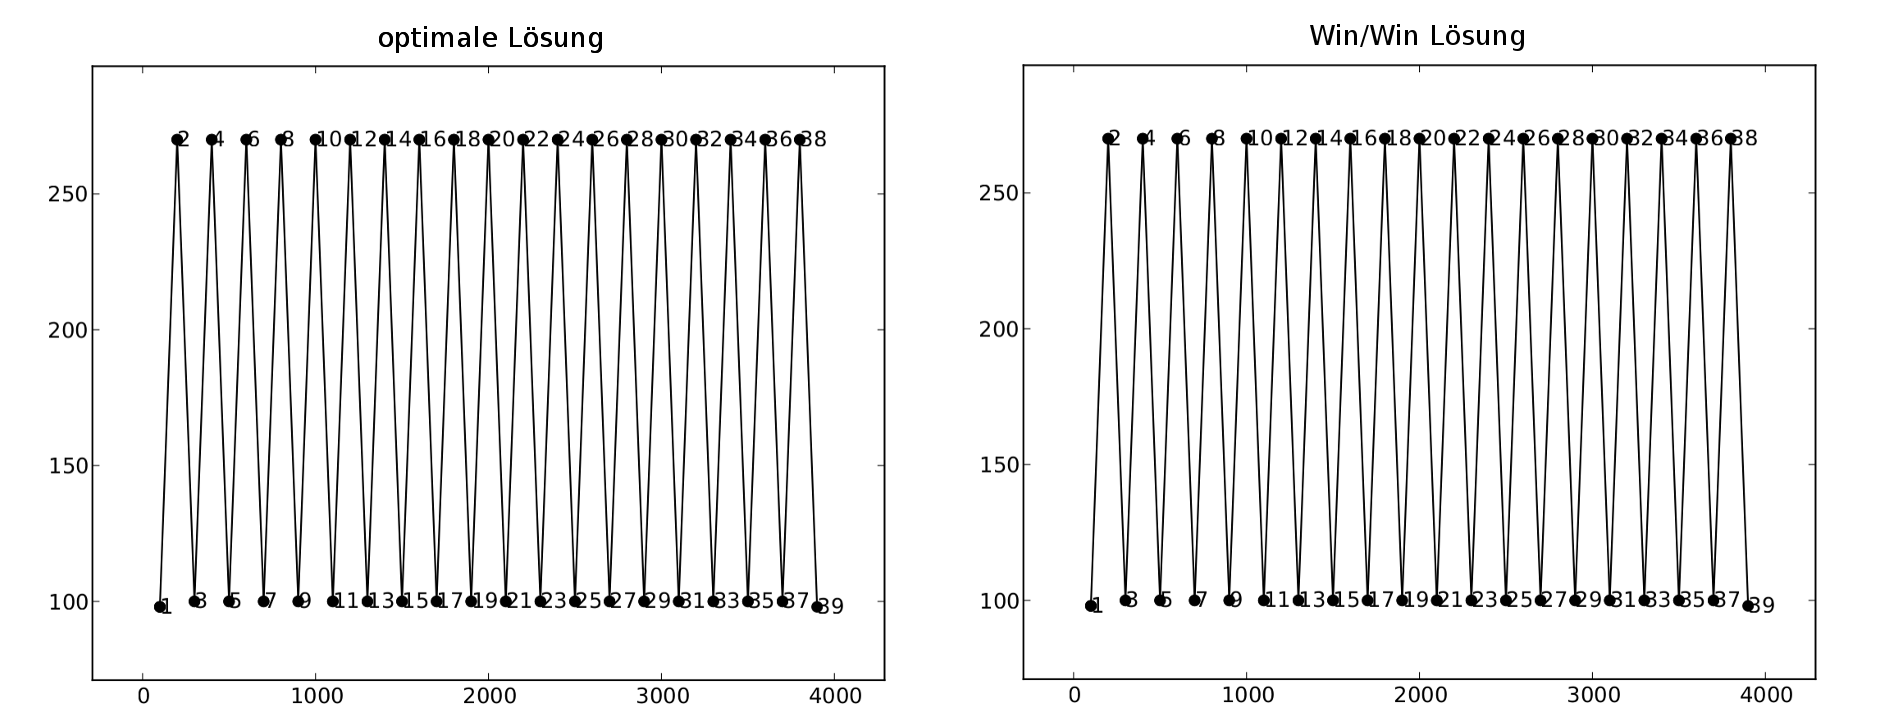
\includegraphics[width=16cm]{gfx/christofides_hpp_comparison}
        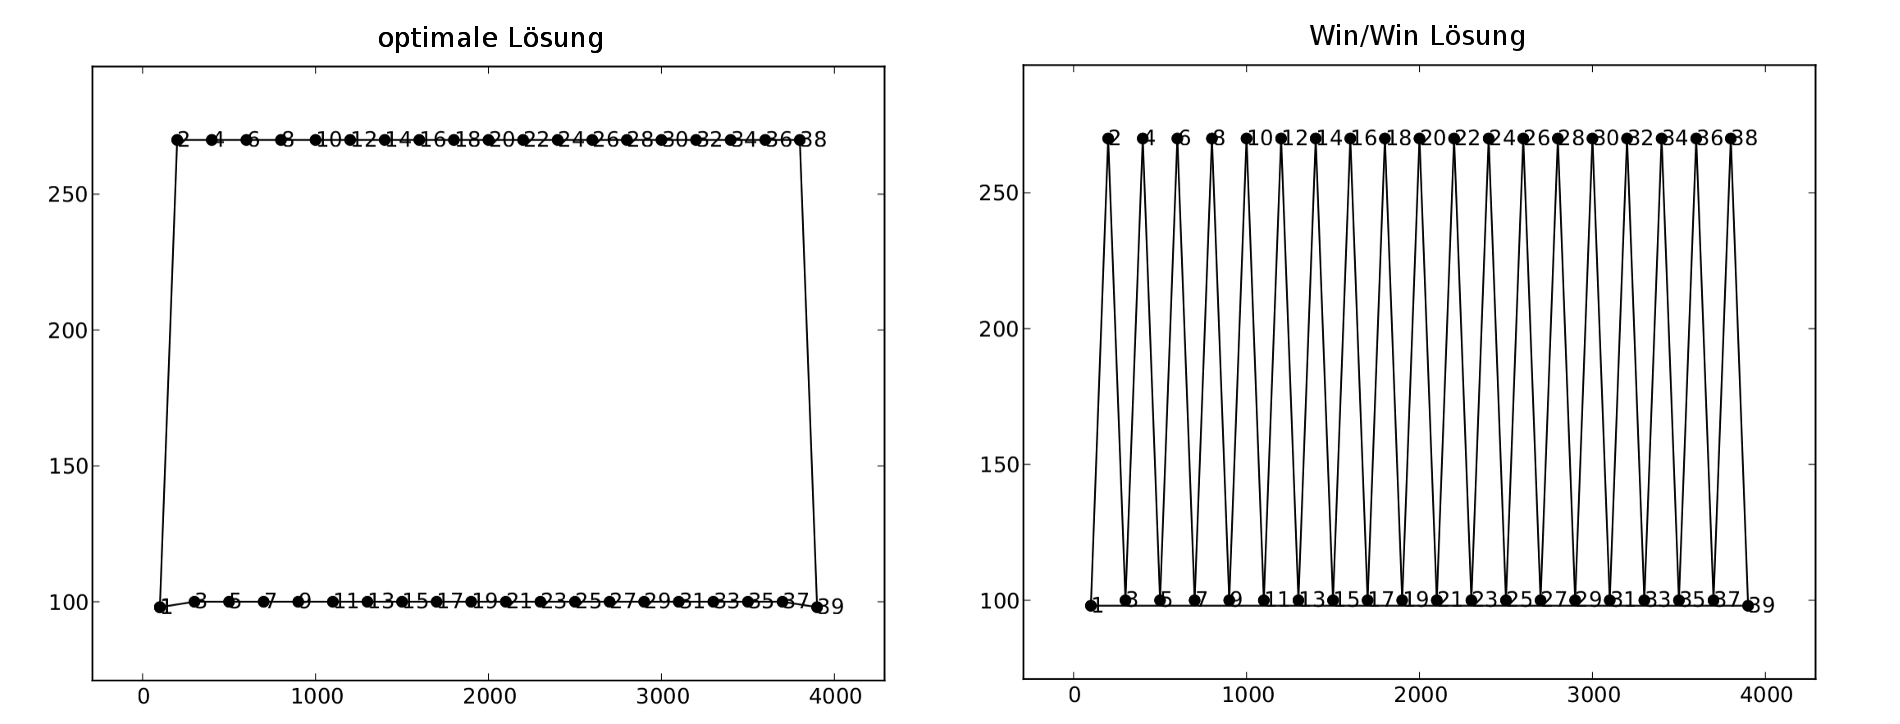
\includegraphics[width=16cm]{gfx/christofides_tsp_comparison}
        \caption{Christofides Instanz}
        \label{img:christofides_comparison}
\end{figure}

\subsubsection{Hoogeveen}
In seinem Paper "`Analysis of Christofides' heuristic: some paths are more difficult than cycles"'\cite{hoogeveen91} zeigte J.A. Hoogeveen anhand dieser Instanz den Worst Case Fall für das Hamiltonpfadproblem.

\begin{table}[H]
        \centering
        \begin{tabular}{| l | r |}
            \hline
                Anzahl Städte               & 8             \\ \hline
                Dimensionen                 & 2             \\ \hline
                Länge optimale Lösung TSP   & 4223          \\ \hline
                Länge Win/Win Lösung  TSP   & 4282          \\ \hline
                Abweichung TSP              & 1.40\%        \\ \hline
                $s$ und $t$ für HPP         & 1, 8          \\ \hline
                Länge optimale Lösung HPP   & 3221          \\ \hline
                Länge Win/Win Lösung  HPP   & 5163          \\ \hline
                Abweichung HPP              & 60.29\%       \\ \hline
        \end{tabular}
        \caption{Instanz Hoogeveen}
        \label{tab:instanz_hoogeveen}
\end{table}

Die Ergebnisse entsprechen den Erwartungen, mit eine Abweichung von 60.29\% liegt das Ergebnis des Hoogeveen Algorithmus nur 6.38 Prozentpunkte unterhalb der oberen Schranke. Auch hier wurde die Instanz leicht verändert, um die schlechten Lösungen zu garantieren.
%TODO: Prozen oder Prozenpunkte => Formulierung prüfen

\begin{figure}[H]
        \centering
        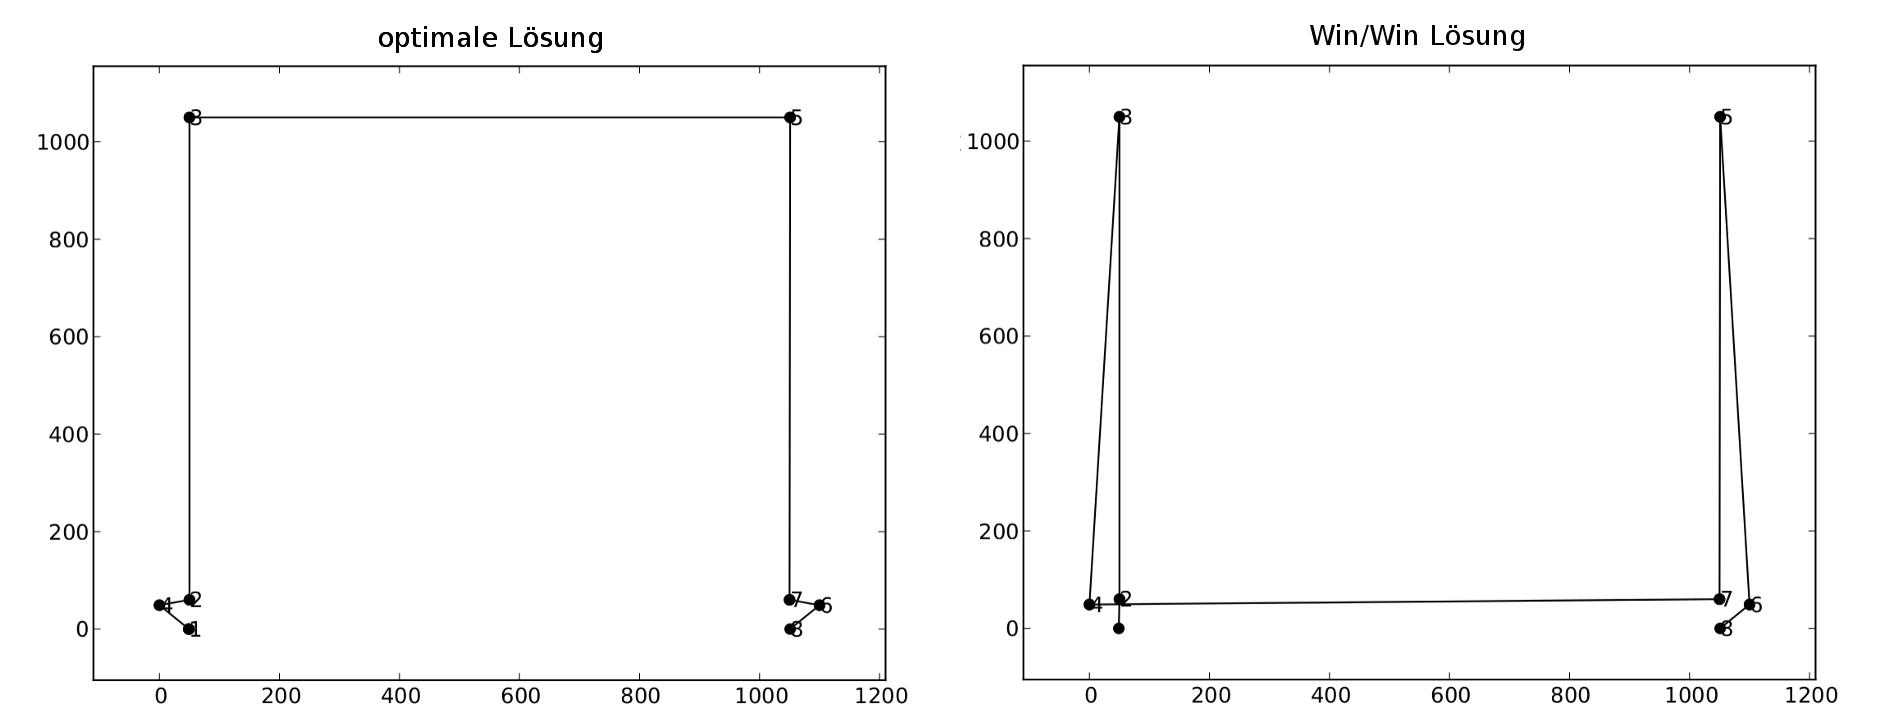
\includegraphics[width=16cm]{gfx/hoogeveen_hpp_comparison}
        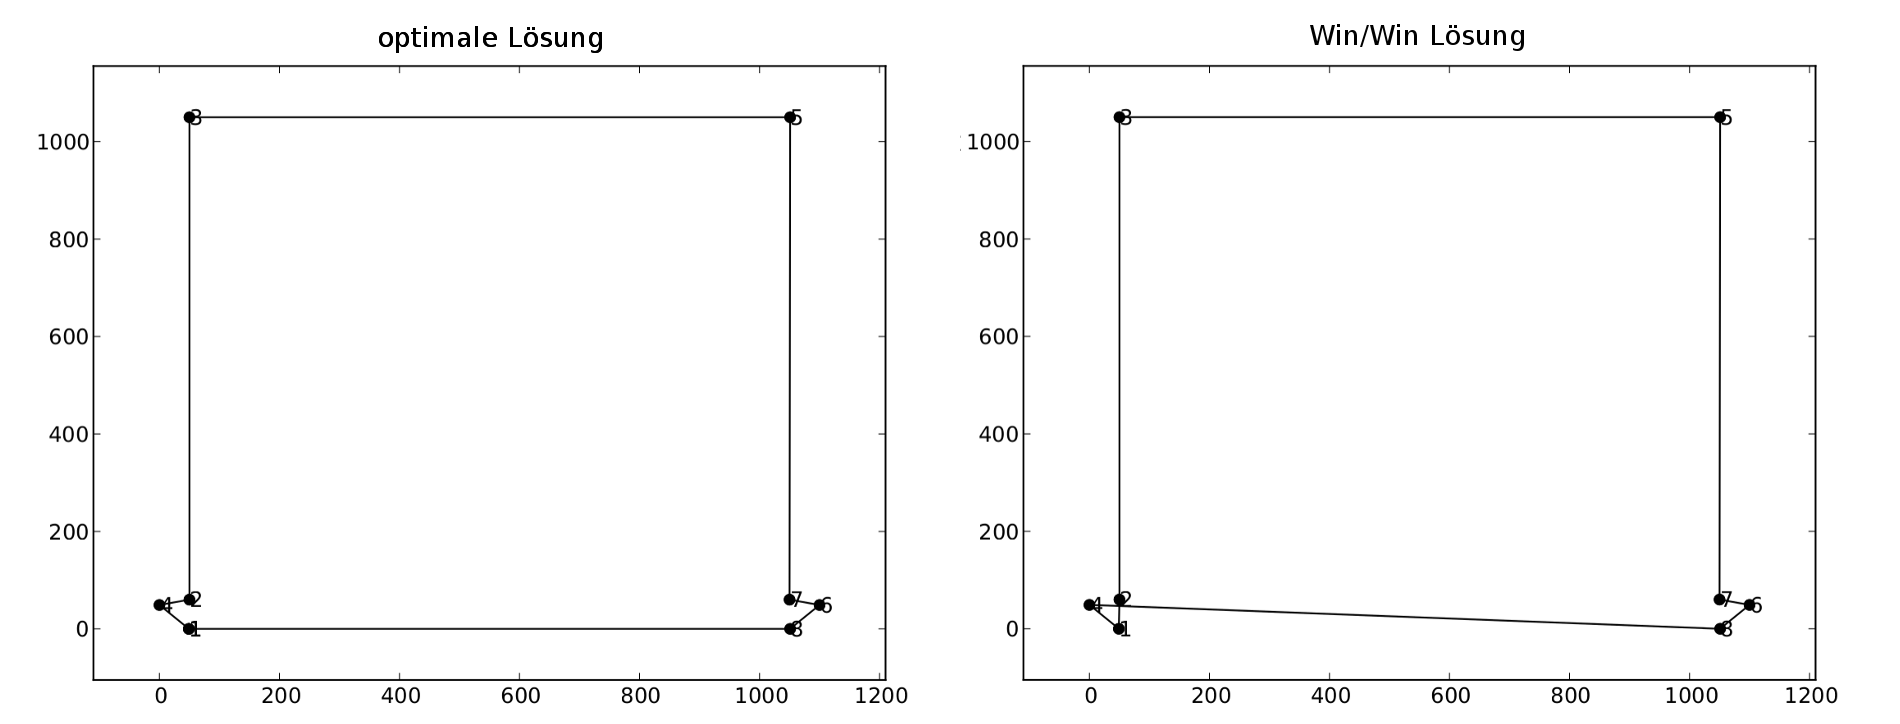
\includegraphics[width=16cm]{gfx/hoogeveen_tsp_comparison}
        \caption{Hoogeveen Instanz}
        \label{img:hoogeveen_comparison}
\end{figure}

\subsubsection{Random 2D-5D}
Eine 50-Städte Instanz mit zufälliger Verteilung. Dazu wurden pro Stadt fünf zufällige Zahlen zwischen 1 und 1000 erzeugt (die Koordinaten der Stadt). Anschliessend wurde auf Grund dieser Koordinaten der Euklidische Abstand der Städte zueinander errechnet.

\begin{table}[H]
        \centering
        \begin{tabular}{| l | r | r | r | r |}
            \hline
            Instanz                     & \textbf{random\_2d}
                                        & \textbf{random\_3d}
                                        & \textbf{random\_4d}
                                        & \textbf{random\_5d} \\ \hline
            Anzahl Städte               & 50        & 50        & 50        & 50            \\ \hline
            Dimensionen                 & 2         & 3         & 4         & 5       \\ \hline
            \o\ Länge optimale Lösung TSP   & 5732.97   & 11075.87  & 16131.26  & 21071.25  \\ \hline
            \o\ Länge Win/Win Lösung  TSP   & 6329.3    & 12232.04  & 17757.49  & 23119.57  \\ \hline
            \o\ Abweichung TSP              & 10.40\%   & 10.44\%   & 10.08\%   & 9.72\%    \\ \hline
            \o\ Länge optimale Lösung HPP   & 5328.47   & 10499.64  & 15419.89  & 20226.01  \\ \hline
            \o\ Länge Win/Win Lösung  HPP   & 5981.15   & 11741.98  & 17104.14  & 22291.39  \\ \hline
            \o\ Abweichung HPP              & 12.24\%   & 11.83\%   & 10.92\%   & 10.21\%   \\ \hline
        \end{tabular}
        \caption{Instanzen Random 2D-5D}
        \label{tab:instanzen_random}
\end{table}

Bei einer zufälligen Verteilung von Knoten ist weder der Christofides, noch der Hoogeveen Algorithmus im Vorteil. Was jedoch auffällt ist, dass die Ergebnisse für beide Algorithmen für höhere Dimensionen genauer werden.

Dies könnte darauf zurückzuführen sein, dass bei höheren Dimensionen die Distanz zwischen den Punkte immer ähnlicher wird. Dass also der Unterschied zwischen der kleinsten und der grössten Distanz im Vergleich zur kleinsten Distanz mit zunehmender Dimension gegen 0 konvergiert.\cite{beyer99}

Wenn nun die Distanzen zwischen den Punkten kaum voneinander abweichen, spielt die gewählte Route eine immer kleinere Rolle.

\begin{figure}[H]
    \centering
    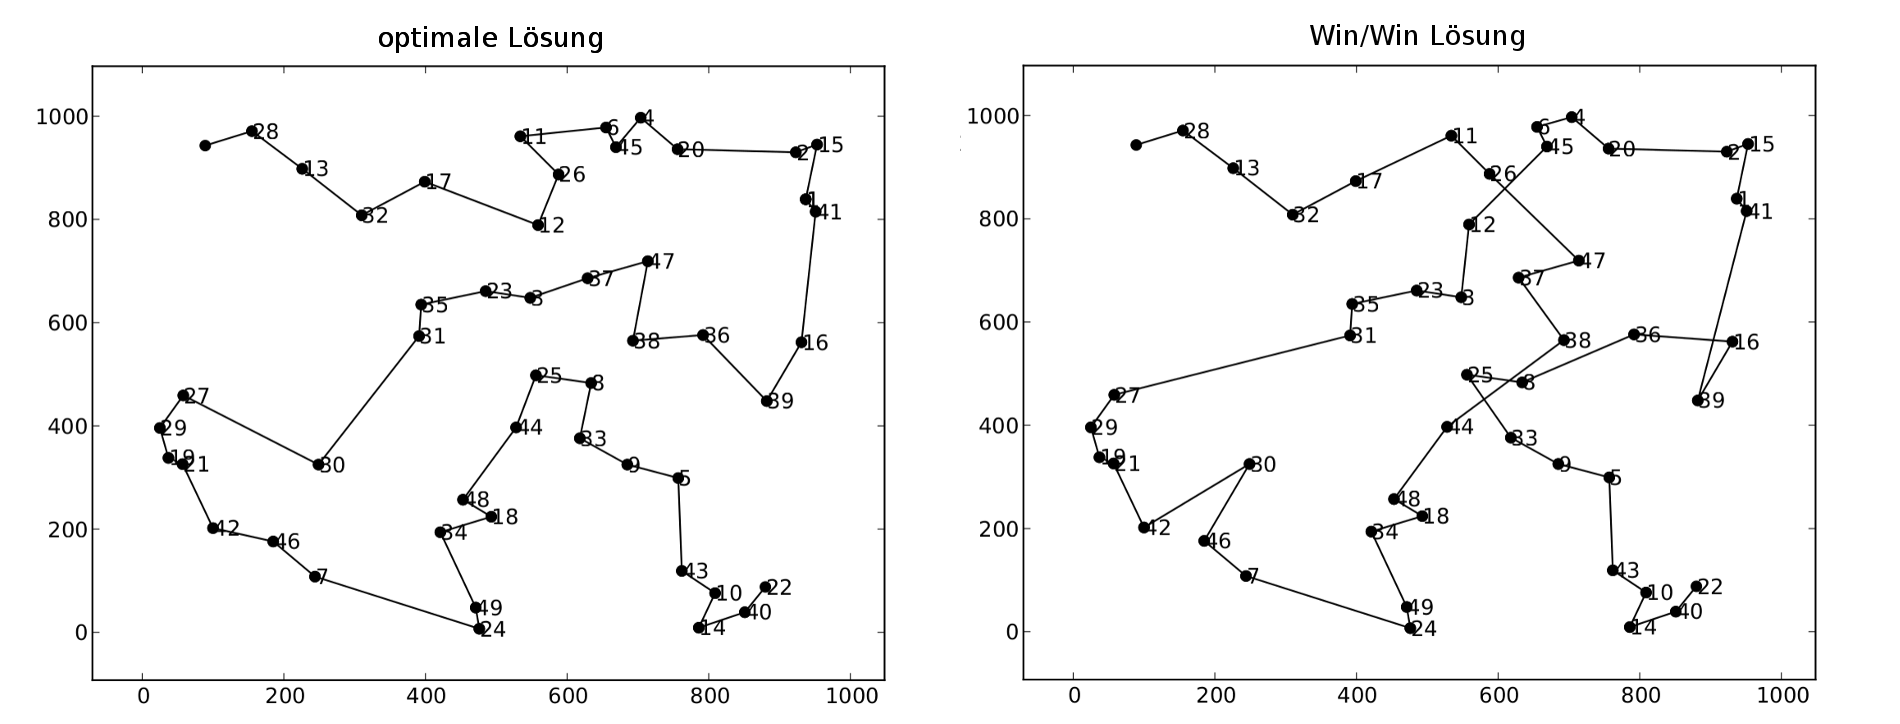
\includegraphics[width=16cm]{gfx/random_hpp_comparison}
    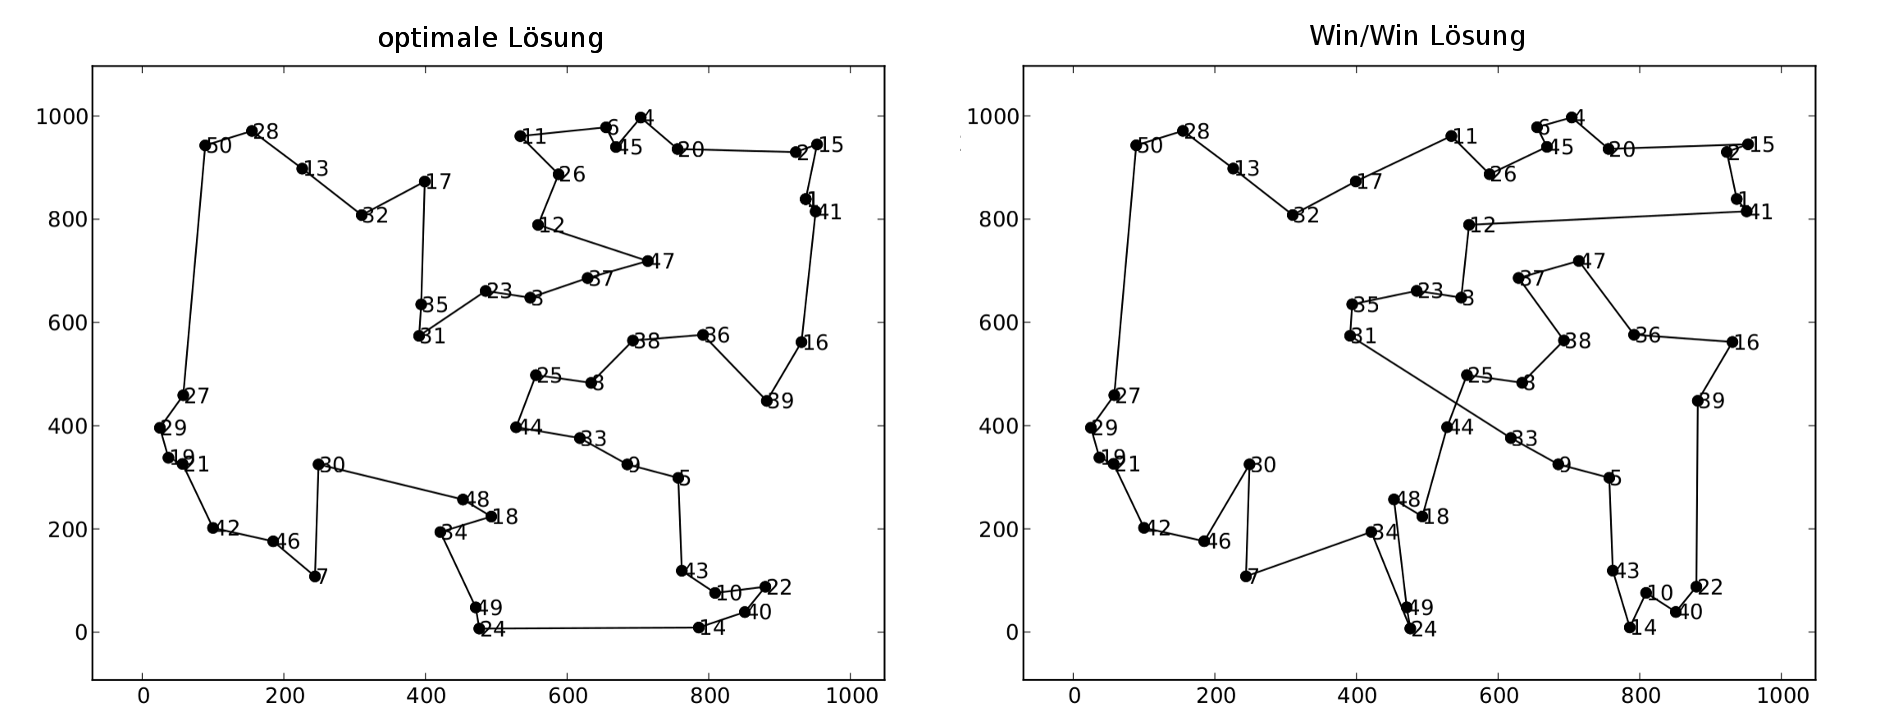
\includegraphics[width=16cm]{gfx/random_tsp_comparison}
    \caption{Random Instanz 2D}
    \label{img:random_comparison}
\end{figure}

\subsubsection{Band 2D-5D}
%TODO: Neu rechnen
Bei dieser Instanz werden die Knoten auf einem länglichen Band verteilt. Dazu werden Städte zwischen zwischen 1 und 100 auf einer Achse und zwischen 1 und 1500 auf den verbleibenden Achsen platziert.

\begin{table}[H]
        \centering
        \begin{tabular}{| l | r | r | r | r |}
            \hline
            Instanz                     & \textbf{band\_2d}     
                                        & \textbf{band\_3d}     
                                        & \textbf{band\_4d}     
                                        & \textbf{band\_5d}             \\ \hline
                Anzahl Städte               & 50        & 50       & 50         & 50        \\ \hline
                Dimensionen                 & 2         & 3        & 4          & 5         \\ \hline
                Länge optimale Lösung TSP   & 3150      & 8861     & 16808      & 25774     \\ \hline
                Länge Win/Win Lösung  TSP   & 3454      & 9646     & 18242      & 28910     \\ \hline
                Abweichung TSP              & 9.65\%    & 10.56\%  & 15.84\%    & 16.51\%   \\ \hline
                $s$ und $t$ für HPP         & 2, 36     & 22, 33   & 19, 31     & 13, 21    \\ \hline
                Länge optimale Lösung HPP   & 2092      & 8266     & 15690      & 24814     \\ \hline
                Länge Win/Win Lösung  HPP   & 2118      & 9095     & 18175      & 27639     \\ \hline
                Abweichung HPP              & 1.24\%    & 8.60\%   & 8.53\%     & 11.38\%   \\ \hline
        \end{tabular}
        \caption{Instanzen Band 2D-5D}
        \label{tab:instanzen_belt}
\end{table}

\begin{figure}[H]
    \centering
    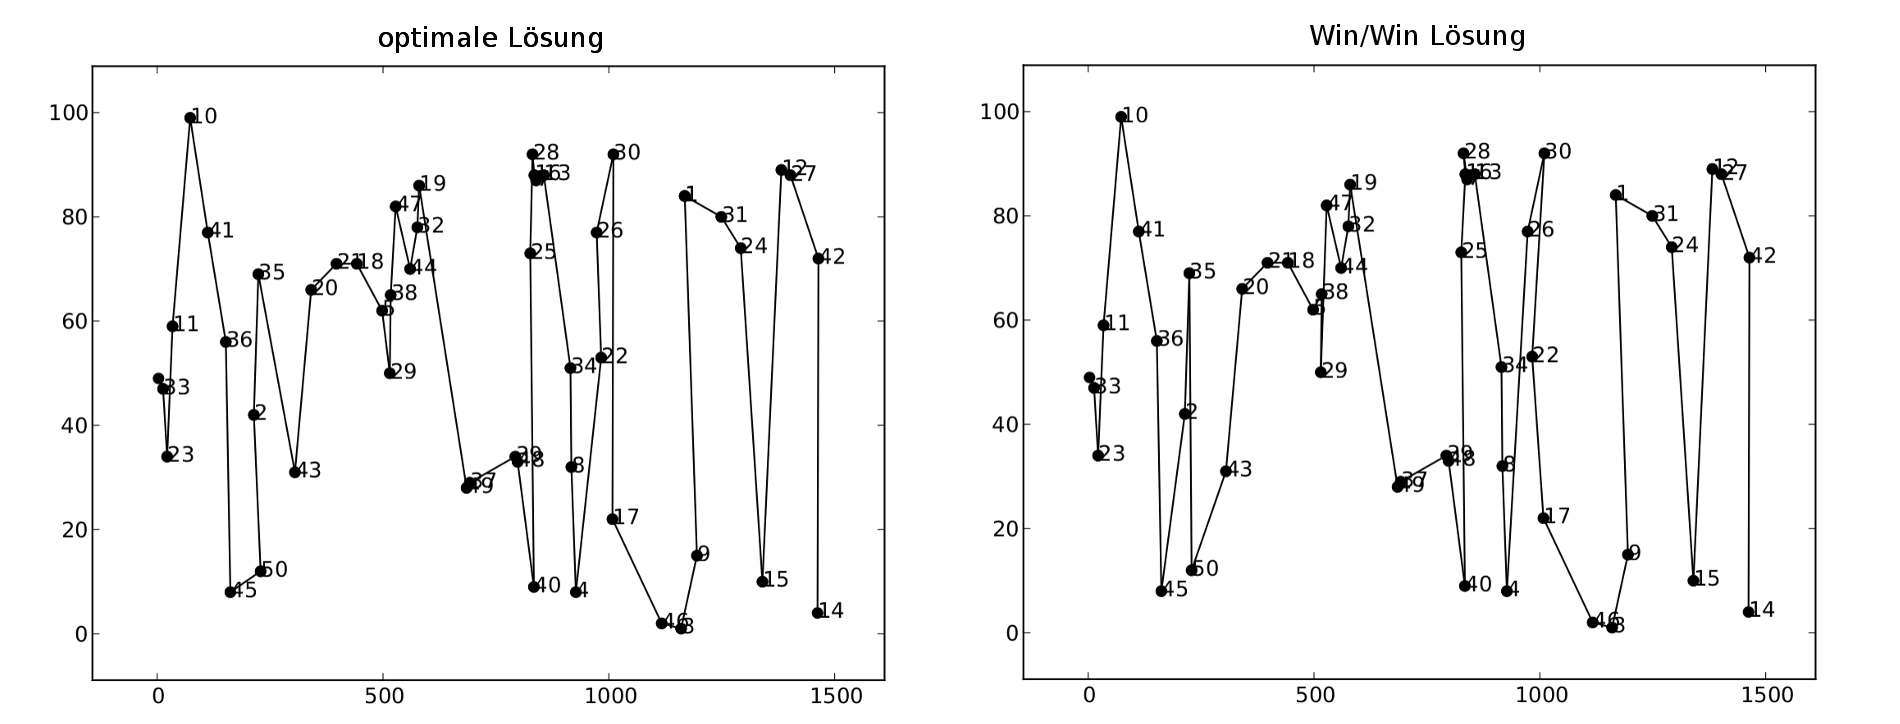
\includegraphics[width=16cm]{gfx/belt_hpp_comparison}
    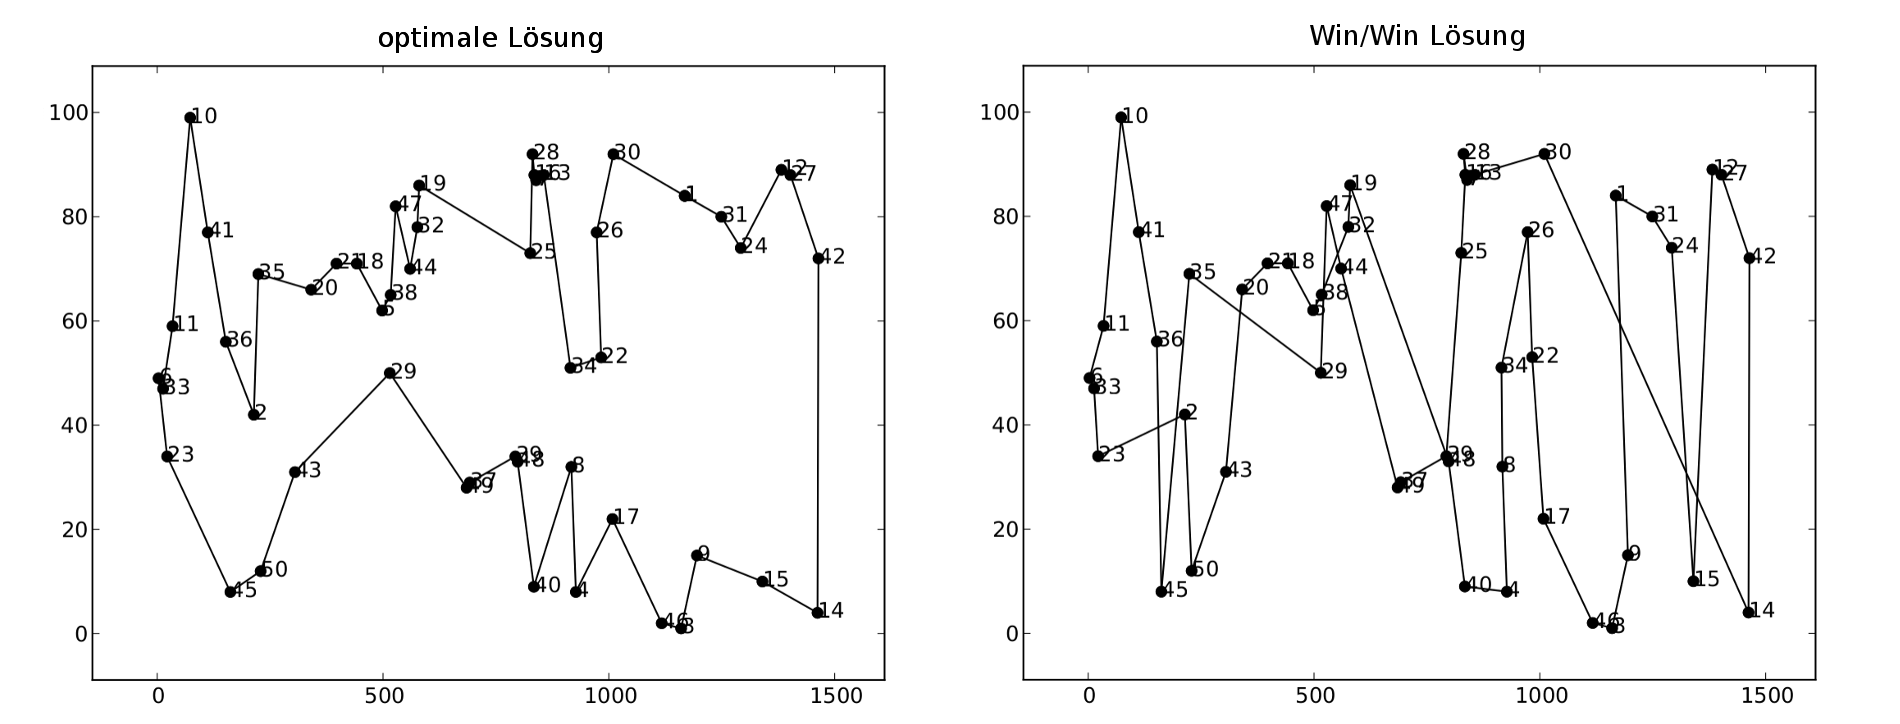
\includegraphics[width=16cm]{gfx/belt_tsp_comparison}
    \caption{Band Instanz 2D}
    \label{img:belt_comparison}
\end{figure}

\subsubsection{Zwei Gruppen 2D-5D}
%TODO: Neu rechnen
Bei dieser Instanz werden die Städte innerhalb zwei definierter Quadrate, bzw. Würfel verteilt. Die Quadrate/Würfel liegen 2000 Einheiten auseinander. Die Quadrate selbst haben eine Seitenlänge von 100 Einheiten.

\begin{table}[H]
        \centering
        \begin{tabular}{| l | r | r | r | r |}
            \hline
            Instanz                     & \textbf{crowds2\_2d}     
                                        & \textbf{crowds2\_3d}     
                                        & \textbf{crowds2\_4d}     
                                        & \textbf{crowds2\_5d}             \\ \hline
                Anzahl Städte               & 50        & 50       & 50         & 50        \\ \hline
                Dimensionen                 & 2         & 3        & 4          & 5         \\ \hline
                Länge optimale Lösung TSP   &           &          &            &           \\ \hline
                Länge Win/Win Lösung  TSP   &           &          &            &           \\ \hline
                Abweichung TSP              &     \%    &      \%  &      \%    &      \%   \\ \hline
                Länge optimale Lösung HPP   &           &          &            &           \\ \hline
                Länge Win/Win Lösung  HPP   &           &          &            &           \\ \hline
                Abweichung HPP              &     \%    &     \%   &     \%     &      \%   \\ \hline
        \end{tabular}
        \caption{Instanzen zwei Gruppen 2D-5D}
        \label{tab:instanzen_crowds2}
\end{table}

\begin{figure}[H]
    \centering
    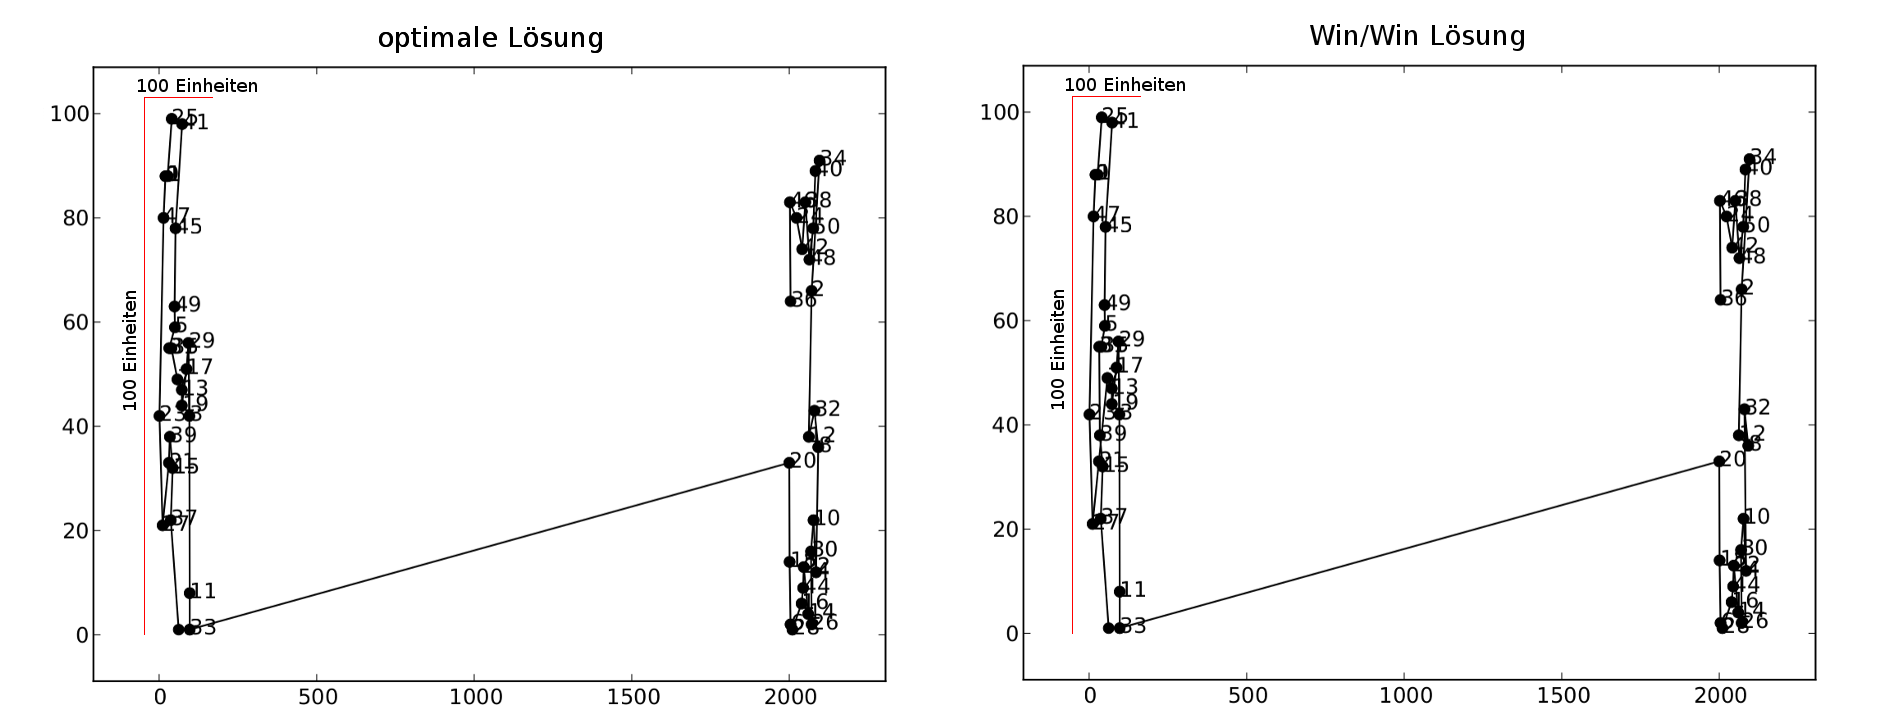
\includegraphics[width=16cm]{gfx/crowds2_hpp_comparison}
    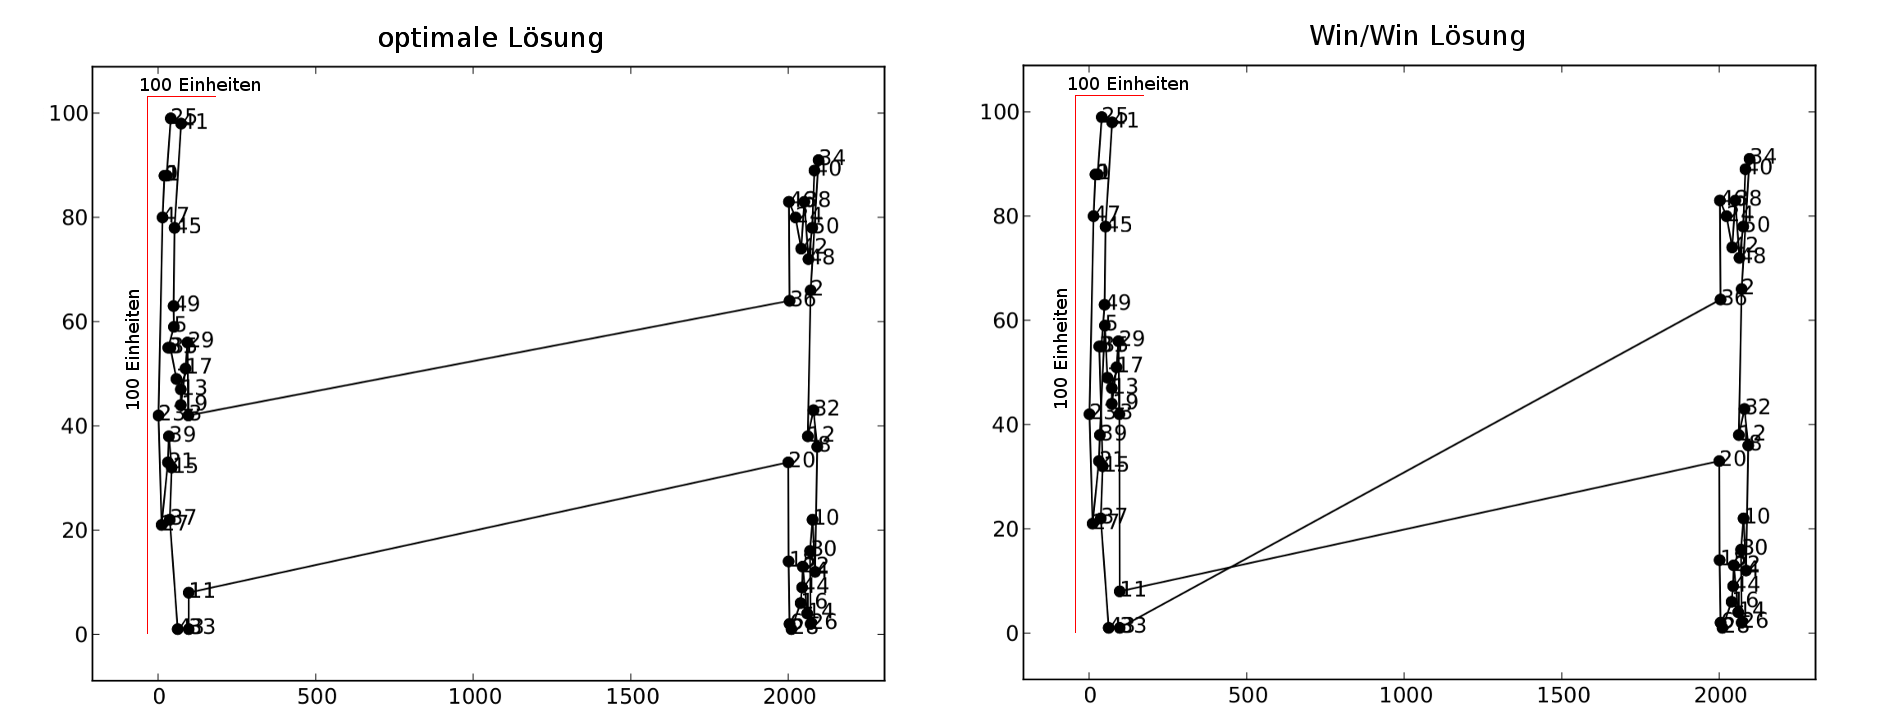
\includegraphics[width=16cm]{gfx/crowds2_tsp_comparison}
    \caption{zwei Gruppen Instanz 2D}
    \label{img:crowds2_comparison}
\end{figure}

\subsubsection{Drei Gruppen 2D-5D}
Bei dieser Instanz werden die Städte innerhalb drei definierter Quadrate verteilt. Die Quadrate liegen 2000 Einheiten auseinander. Die Quadrate selbst haben eine Seitenlänge von 100 Einheiten.

\begin{table}[H]
        \centering
        \begin{tabular}{| l | r | r | r | r |}
            \hline
            Instanz                     & \textbf{crowds3\_2d}     
                                        & \textbf{crowds3\_3d}     
                                        & \textbf{crowds3\_4d}     
                                        & \textbf{crowds3\_5d}             \\ \hline
                Anzahl Städte               & 50        & 50       & 50         & 50        \\ \hline
                Dimensionen                 & 2         & 3        & 4          & 5         \\ \hline
                Länge optimale Lösung TSP   &           &          &            &           \\ \hline
                Länge Win/Win Lösung  TSP   &           &          &            &           \\ \hline
                Abweichung TSP              &     \%    &      \%  &      \%    &      \%   \\ \hline
                Länge optimale Lösung HPP   &           &          &            &           \\ \hline
                Länge Win/Win Lösung  HPP   &           &          &            &           \\ \hline
                Abweichung HPP              &     \%    &     \%   &     \%     &      \%   \\ \hline
        \end{tabular}
        \caption{Instanzen drei Gruppen 2D-5D}
        \label{tab:instanzen_crowds3}
\end{table}

\subsubsection{Zusammenfassung}
    \begin{table}[H]
                \centering
                \begin{tabular}{| p{2.0cm} | p{2.0cm} | p{2.5cm} | p{2.5cm} | p{2.5cm} |}
                    \hline
                    \small{\textbf{Name}} &
                    \small{\textbf{Anzahl Städte}}  & 
                    \small{\textbf{Dimensionen}} & 
                    \small{\textbf{Abweichung TSP}} & 
                    \small{\textbf{Abweichung HPP}} \\ \hline

                    christofides    & 39    & 2     & 44.78\%   & 0\%           \\ \hline
                    hoogeveen       & 8     & 2     & 1.68\%    & 61.56\%       \\ \hline
                    random\_2d      & 50    & 2     & 13.40\%   & 15.45\%       \\ \hline
                    random\_3d      & 50    & 3     & 15.17\%   & 17.81\%       \\ \hline
                    random\_4d      & 50    & 4     & 6.88\%    & 9.40\%        \\ \hline
                    random\_5d      & 50    & 5     & 9.82\%    & 7.65\%        \\ \hline
                    band\_2d        & 50    & 2     & 9.65\%    & 1.24\%        \\ \hline
                    band\_3d        & 50    & 3     & 10.56\%   & 8.60\%        \\ \hline
                    band\_4d        & 50    & 4     & 15.84\%   & 8.53\%        \\ \hline
                    band\_5d        & 50    & 5     & 16.51\%   & 11.38\%       \\ \hline
               \end{tabular}
                \caption{Auswertung der eigenen Instanzen}
                \label{tab:instanz_eigene_instanzen}
        \end{table}

\newpage

\section{Fazit}
\subsection{Rückblick}
\subsection{Weitere Möglichkeiten}

\newpage

% bibliography
\bibliographystyle{plain}
\bibliography{bibliographie}
\end{document}
